\documentclass[11pt,a4paper]{article}
\usepackage[margin=2.5cm]{geometry}
\usepackage{enumitem}
\usepackage{titlesec}
\usepackage{hyperref}
\usepackage{xcolor}
\usepackage{booktabs}
\usepackage{parskip}
\usepackage{graphicx}
\usepackage{amsmath}
\usepackage{float}
\usepackage{listings}
\usepackage{tcolorbox}
\tcbuselibrary{listings,breakable,skins}

\definecolor{accent}{RGB}{30,70,120}
\definecolor{gold}{RGB}{140,110,30}
\definecolor{green}{RGB}{40,120,40}
\definecolor{red}{RGB}{180,40,40}
\definecolor{codebg}{RGB}{245,245,245}
\definecolor{codeframe}{RGB}{200,200,200}
\definecolor{codekw}{RGB}{0,100,170}
\definecolor{codecomment}{RGB}{100,130,100}
\definecolor{codestr}{RGB}{170,55,55}

\lstdefinestyle{python}{
    language=Python,
    basicstyle=\ttfamily\footnotesize,
    keywordstyle=\color{codekw}\bfseries,
    commentstyle=\color{codecomment}\itshape,
    stringstyle=\color{codestr},
    showstringspaces=false,
    breaklines=true,
    breakatwhitespace=true,
    tabsize=4,
    numbers=left,
    numberstyle=\tiny\color{gray},
    numbersep=8pt,
}

\lstdefinestyle{shell}{
    language=bash,
    basicstyle=\ttfamily\footnotesize,
    keywordstyle=\color{codekw},
    commentstyle=\color{codecomment}\itshape,
    showstringspaces=false,
    breaklines=true,
    breakatwhitespace=true,
    tabsize=4,
    numbers=none,
}

% ── Result highlight boxes (inspired by matthieu-katya.pdf) ────────
\definecolor{strongbg}{RGB}{230,245,230}      % green tint
\definecolor{strongframe}{RGB}{60,140,60}
\definecolor{promisingbg}{RGB}{255,250,230}    % amber tint
\definecolor{promisingframe}{RGB}{180,150,40}
\definecolor{failbg}{RGB}{255,235,235}         % red tint
\definecolor{failframe}{RGB}{180,60,60}
\definecolor{neutralbg}{RGB}{240,245,255}      % blue tint
\definecolor{neutralframe}{RGB}{80,110,170}

\newtcolorbox{resultbox}[2][]{
    enhanced,
    colback=#2bg,
    colframe=#2frame,
    boxrule=0.8pt,
    arc=3pt,
    left=6pt, right=6pt, top=4pt, bottom=4pt,
    fonttitle=\bfseries\color{#2frame},
    title={#1},
    breakable,
}

\newtcolorbox{codebox}[1][]{
    colback=codebg,
    colframe=codeframe,
    boxrule=0.5pt,
    arc=2pt,
    left=2pt,
    right=2pt,
    top=2pt,
    bottom=2pt,
    breakable,
    title={\small\ttfamily #1},
    fonttitle=\bfseries\color{accent},
}

\titleformat{\section}{\large\bfseries\color{accent}}{}{0em}{}[\titlerule]
\titleformat{\subsection}{\normalsize\bfseries\color{accent}}{}{0em}{}

\hypersetup{
    colorlinks=true,
    linkcolor=accent,
    urlcolor=accent
}

\setcounter{tocdepth}{2}

\begin{document}

% ══════════════════════════════════════════════════════════════════
% TITLE PAGE
% ══════════════════════════════════════════════════════════════════

\begin{center}
\vspace*{3cm}
{\Huge\bfseries\color{accent} The Bookmaker's Edge}\\[1em]
{\LARGE Momentum Timing Across\\[0.3em]
Bitcoin, Gold, Silver, Oil, Gas, and Copper}\\[2em]
{\large Robin Langer}\\[0.5em]
{\small August 2026}\\[3em]
\textit{``When you have nothing, you need a mechanism\\
that doesn't depend on what you have.''}
\vspace*{2cm}
\end{center}

\thispagestyle{empty}
\newpage

% ══════════════════════════════════════════════════════════════════
% EXECUTIVE SUMMARY
% ══════════════════════════════════════════════════════════════════

\section*{Executive Summary}
\addcontentsline{toc}{section}{Executive Summary}

This report tests the \textbf{bookmaker-pool momentum model} ---
originally developed for ASX equities --- across seven asset classes:
cryptocurrency, precious metals, energy commodities, industrial
metals, equity indices, and foreign exchange.

The model computes a ``momentum price'' from volume-weighted flows
and compares it to the market price. When momentum price $>$ market
price, hold. When momentum price $<$ market price, go to cash.

\vspace{0.5em}
\begin{tabular}{@{}llrl@{}}
    \toprule
    \textbf{Asset Class} & \textbf{Best Ticker} & \textbf{Alpha} & \textbf{Verdict} \\
    \midrule
    Cryptocurrency   & SOL-USD (180d)  & \textcolor{green}{\textbf{+2597\%}} & Monster: best in class \\
    Cryptocurrency   & BTC-USD (180d)  & \textcolor{green}{\textbf{+295\%}}  & Strong: trade this \\
    Energy           & Nat Gas NG=F (90d) & \textcolor{green}{\textbf{+299\%}} & Strong: all lookbacks work \\
    Precious Metals  & Silver SI=F (180d) & $+68\%$\textsuperscript{*} & Promising (recent) \\
    Industrial Metals& Copper HG=F (180d) & $+15\%$  & Good risk-adjusted \\
    Energy           & Crude Oil CL=F (90d) & $+32\%$ & Risk mgmt only \\
    Precious Metals  & Gold GC=F (180d) & $-182\%$  & Risk mgmt only \\
    Forex            & EUR 6E=F (180d)  & $+11\%$   & Risk mgmt only \\
    Cryptocurrency   & ETH-USD (180d)   & $-155\%$  & Don't trade \\
    Equity Index     & ES=F (180d)      & $-98\%$   & Broken: don't use \\
    \bottomrule
\end{tabular}

\vspace{0.3em}
{\small \textsuperscript{*}Silver alpha is from the recent 2021--2026 period; 16-year alpha is $-51\%$.}

\vspace{0.5em}
\textbf{Key findings:}

\begin{enumerate}[leftmargin=2em]
    \item \textbf{SOL is the monster.} +7691\% return vs +5094\%
          buy \& hold, Sharpe 1.34, max drawdown cut from $-96\%$ to
          $-79\%$. The model thrives on extreme volatility.
    \item \textbf{Natural gas has positive alpha on all lookbacks}
          --- the only asset to achieve this. 90-day: +299\%, 180-day:
          +163\%, 365-day: +84\%.
    \item \textbf{Copper is the quiet achiever.} Sharpe 1.05, 100\%
          win rate (6/6 trades), max drawdown cut from $-35\%$ to $-23\%$.
    \item \textbf{BTC remains the flagship.} +462\% return, Sharpe
          1.16, 14:1 win/loss asymmetry.
    \item \textbf{180-day lookback is optimal for most assets.} Across
          crypto, metals, and forex, 180 days wins. Exception: energy
          commodities, where 90 days produces higher returns.
    \item \textbf{Drawdown reduction is universal.} Even where the
          strategy underperforms on return, it consistently halves
          max drawdown.
    \item \textbf{Equity indices don't work.} The S\&P 500's structural
          upward drift keeps the momentum ratio permanently below 1.
          The model sits in cash 99\% of the time.
\end{enumerate}

\newpage

% ══════════════════════════════════════════════════════════════════
% TABLE OF CONTENTS
% ══════════════════════════════════════════════════════════════════

\tableofcontents
\newpage

% ══════════════════════════════════════════════════════════════════
% PART I: THE MODEL
% ══════════════════════════════════════════════════════════════════

\part{The Model}

\section{The Intuition: A Day at the Races}

Before the mathematics, consider a horse race.

\subsection{The Bookmaker's Pool}

A bookmaker doesn't set the odds himself --- the \emph{punters} do,
by where they put their money. Suppose three horses are running in
the Melbourne Cup, and the total pool is \$100,000:

\vspace{0.5em}
\begin{tabular}{@{}lrrr@{}}
    \toprule
    \textbf{Horse} & \textbf{Money bet} & \textbf{Share of pool}
        & \textbf{Implied odds} \\
    \midrule
    Thunderbolt  & \$60,000 & 60\% & 1.67 to 1 (\$0.67 profit per \$1) \\
    Silver Arrow & \$30,000 & 30\% & 3.33 to 1 (\$2.33 profit per \$1) \\
    Dark Horse   & \$10,000 & 10\% & 10 to 1 (\$9.00 profit per \$1) \\
    \midrule
    \textbf{Total pool} & \textbf{\$100,000} & \textbf{100\%} & \\
    \bottomrule
\end{tabular}

\vspace{0.5em}
The odds tell you what the \emph{crowd} thinks. Thunderbolt is the
favourite because the most money backs it. But here's the key insight:
\textbf{the odds keep changing as more money comes in.}

Suppose a rumour spreads that Dark Horse had a secret training session
and looked incredible. Suddenly, \$20,000 of new money pours in on
Dark Horse:

\vspace{0.5em}
\begin{tabular}{@{}lrrr@{}}
    \toprule
    \textbf{Horse} & \textbf{Money bet} & \textbf{Share of pool}
        & \textbf{Implied odds} \\
    \midrule
    Thunderbolt  & \$60,000 & 50\% & 2.0 to 1 \\
    Silver Arrow & \$30,000 & 25\% & 4.0 to 1 \\
    Dark Horse   & \$30,000 & 25\% & 4.0 to 1 \\
    \midrule
    \textbf{Total pool} & \textbf{\$120,000} & \textbf{100\%} & \\
    \bottomrule
\end{tabular}

\vspace{0.5em}
Dark Horse's odds have shortened from 10:1 to 4:1. Not because the
bookmaker decided it was faster --- but because \emph{the money moved}.
The pool reflects the collective conviction of everyone with skin in
the game.

\subsection{From Horses to Markets}

Now replace the horses with an asset --- Bitcoin, gold, silver, a
stock. Each trading day, people place their bets:

\begin{itemize}[leftmargin=2em]
    \item \textbf{Buyers} put money into the pool (they think the price
          should be higher).
    \item \textbf{Sellers} take money out (they think the price should
          be lower).
    \item The \textbf{volume} tells you how much money moved.
    \item The \textbf{daily return} tells you which direction it moved.
\end{itemize}

On a day when Bitcoin rises 3\% on heavy volume, that's like a rush
of money pouring in on Thunderbolt --- a large, high-conviction bet
that the price should be higher. On a day when Bitcoin falls 2\% on
light volume, that's like a few punters nervously pulling money off
Silver Arrow --- a small, low-conviction bet that the price should
be lower.

The \textbf{momentum price} is what the pool says the asset is worth,
after accumulating all these daily bets over time. If the pool says
``\$110,000'' but the market price is \$95,000, then the weight of
money --- the collective conviction of everyone who has traded ---
supports a higher price. The asset is \textbf{undervalued by momentum}.

That's when you buy.

If the pool says ``\$80,000'' but the market price is \$95,000, the
money has been flowing out. The crowd is quietly leaving. The asset is
\textbf{overvalued by momentum}.

That's when you hold cash and wait.

\section{The Algorithm: Formal Definition}

\subsection{Mathematical Definition}

Given a time series of daily closing prices $P_t$ and volumes $V_t$:

\begin{enumerate}[leftmargin=2em]
    \item Compute daily returns:
          $r_t = \dfrac{P_t - P_{t-1}}{P_{t-1}}$

    \item Normalise volume (to prevent overflow on large numbers):
          $\hat{V}_t = \dfrac{V_t}{\bar{V}}$
          where $\bar{V}$ is the mean volume over the lookback window.

    \item Compute net directional flow:
          $f_t = \hat{V}_t \times r_t$

          On up days ($r_t > 0$), $f_t$ is positive --- buyers are winning.
          On down days ($r_t < 0$), $f_t$ is negative --- sellers are winning.
          On balanced days, the flows cancel out.

    \item Update the pool iteratively:
          \begin{align*}
              \text{pool}_0 &= P_0 \\
              \text{pool}_t &= \text{pool}_{t-1} + f_t \times \text{pool}_{t-1}
          \end{align*}

    \item The momentum price is the final pool value:
          $M = \text{pool}_T$
\end{enumerate}

\subsection{The Signal}

The \textbf{momentum ratio} is:
$$\rho = \frac{M}{P_T}$$

\begin{itemize}[leftmargin=2em]
    \item $\rho > 1$: The volume-weighted flow of money supports a
          \emph{higher} price than the market is offering. The asset is
          \textbf{undervalued} by momentum. \textbf{Hold the asset.}
    \item $\rho < 1$: The volume-weighted flow of money supports a
          \emph{lower} price. The asset is \textbf{overvalued} by
          momentum. \textbf{Hold cash.}
\end{itemize}

The lookback window (how many days of history feed the pool) is a
tunable parameter. We tested 90, 180, and 365 days across all assets.

\subsection{Origin}

This model was originally developed for ASX 100 equities, where it
produced +13.6\% alpha per 6-month period over 10 consecutive periods
(p = 0.046). This report tests whether it transfers to cryptocurrency
and precious metals.

\newpage

% ══════════════════════════════════════════════════════════════════
% PART II: CRYPTOCURRENCY
% ══════════════════════════════════════════════════════════════════

\part{Cryptocurrency}

\section{Experiment 1: BTC/ETH Pairs Trade (Failed)}

\subsection{Hypothesis}

When Bitcoin is over-momentum-priced and Ethereum is
under-momentum-priced simultaneously, rotate from BTC into ETH.
Rotate back when the spread recalibrates. This is a
\textbf{relative value} or \textbf{pairs trade}.

\subsection{Result}

\begin{tabular}{@{}lrr@{}}
    \toprule
    \textbf{Metric} & \textbf{90-day} & \textbf{180-day} \\
    \midrule
    Strategy return    & $-91.1\%$  & $-42.9\%$  \\
    ETH buy \& hold    & $+311.8\%$ & $-21.3\%$  \\
    BTC buy \& hold    & $+305.0\%$ & $+19.7\%$  \\
    Sharpe ratio       & $-0.70$    & $-0.48$    \\
    Max drawdown       & $-94.3\%$  & $-69.1\%$  \\
    Trades             & 11         & 3          \\
    \bottomrule
\end{tabular}

\vspace{0.5em}
\textbf{Verdict: Total failure.} The strategy lost money across every
configuration tested.

\subsection{Why It Failed}

\begin{enumerate}[leftmargin=2em]
    \item \textbf{Correlated momentum signals.} BTC and ETH are driven
          by the same macro forces (interest rates, risk appetite,
          regulatory news). Their momentum ratios move in lockstep.
          The spread between them is noise, not signal.

    \item \textbf{Secular trend.} ETH has been in a structural decline
          against BTC since mid-2022. A mean-reversion strategy on a
          pair that is \emph{not mean-reverting} is guaranteed to lose.

    \item \textbf{The original model works on independent assets.}
          On the ASX, BHP and CSL have genuinely different fundamentals.
          BTC and ETH do not --- they are both ``crypto.''
\end{enumerate}

This approach is \textbf{abandoned}.

\section{Experiment 2: Bitcoin Timing (Strong)}

\subsection{Hypothesis}

Use the momentum ratio as a timing signal on a \textbf{single asset}:
hold when $\rho > 1$ (undervalued), go to cash when
$\rho \leq 1$ (overvalued). No pairs, no shorting --- just timing.

\subsection{Results: Bitcoin (BTC-USD)}

Period: 1 January 2021 to 24 August 2026 (2,062 trading days).

\vspace{0.5em}
\begin{tabular}{@{}lrrr@{}}
    \toprule
    \textbf{Metric} & \textbf{90-day} & \textbf{180-day} & \textbf{365-day} \\
    \midrule
    Strategy return    & $+39.6\%$  & \textcolor{green}{\textbf{+462.7\%}} & $+132.3\%$ \\
    Buy \& hold return & $+167.5\%$ & $+167.5\%$  & $+167.5\%$ \\
    Alpha              & $-127.9\%$ & \textcolor{green}{\textbf{+295.2\%}} & $-35.2\%$  \\
    \midrule
    Sharpe ratio       & $0.35$     & \textcolor{green}{\textbf{1.16}}     & $0.66$     \\
    Max drawdown       & $-59.5\%$  & \textcolor{green}{\textbf{-28.1\%}}  & $-33.2\%$  \\
    Buy \& hold DD     & $-76.6\%$  & $-76.6\%$ & $-76.6\%$ \\
    \midrule
    Days in BTC        & 34.0\%     & 34.3\%     & 30.2\%     \\
    Days in cash       & 66.0\%     & 65.7\%     & 69.8\%     \\
    Distinct trades    & 22         & 16         & 10         \\
    Win rate           & 45\%       & 62\%       & 50\%       \\
    Avg win            & $+14.8\%$  & $+26.8\%$  & $+21.3\%$  \\
    Avg loss           & $-9.2\%$   & $-1.9\%$   & $-3.0\%$   \\
    Crashes avoided    & 3          & 2          & 2          \\
    \bottomrule
\end{tabular}

\vspace{1em}

\begin{resultbox}[Verdict: Bitcoin --- Strong]{strong}
The \textbf{180-day lookback} is the clear winner:
+462.7\% return vs +167.5\% buy \& hold (\textbf{+295.2\% alpha}),
Sharpe 1.16, max drawdown cut from $-76.6\%$ to $-28.1\%$.
Only in the market 34\% of the time. 62\% win rate with a
\textbf{14:1 win/loss asymmetry} (+26.8\% vs $-1.9\%$).
\end{resultbox}

\subsection{Results: Ethereum (ETH-USD)}

\vspace{0.5em}
\begin{tabular}{@{}lr@{}}
    \toprule
    \textbf{Metric} & \textbf{180-day} \\
    \midrule
    Strategy return    & $+86.1\%$  \\
    Buy \& hold return & $+241.4\%$ \\
    Alpha              & $-155.2\%$ \\
    Sharpe ratio       & $0.50$     \\
    Max drawdown       & $-56.0\%$  \\
    Win rate           & 50\%       \\
    \bottomrule
\end{tabular}

\begin{resultbox}[Verdict: Ethereum --- Don't Trade]{fail}
The model \textbf{does not work well on ETH}. It reduces drawdown
but misses too much upside. $-155\%$ alpha. Not recommended.
\end{resultbox}

\subsection{Results: Solana (SOL-USD)}

Period: 1 January 2021 to 24 August 2026 (2,062 trading days).

\vspace{0.5em}
\begin{tabular}{@{}lrrr@{}}
    \toprule
    \textbf{Metric} & \textbf{90-day} & \textbf{180-day} & \textbf{365-day} \\
    \midrule
    Strategy return    & $+6883.5\%$ & \textcolor{green}{\textbf{+7691.4\%}} & $+201.8\%$ \\
    Buy \& hold return & $+5089.2\%$ & $+5094.1\%$  & $+256.2\%$ \\
    Alpha              & $+1794.3\%$ & \textcolor{green}{\textbf{+2597.2\%}} & $-54.4\%$  \\
    \midrule
    Sharpe ratio       & $1.29$      & \textcolor{green}{\textbf{1.34}}      & $0.65$     \\
    Max drawdown       & $-89.9\%$   & $-78.7\%$    & $-86.5\%$  \\
    Buy \& hold DD     & $-96.3\%$   & $-96.3\%$    & $-96.3\%$  \\
    \midrule
    Days in SOL        & 60.3\%      & 55.3\%       & 46.3\%     \\
    Days in cash       & 39.7\%      & 44.7\%       & 53.7\%     \\
    Distinct trades    & 27          & 16           & 23         \\
    Win rate           & 52\%        & 50\%         & 48\%       \\
    Avg win            & $+109.9\%$  & $+204.3\%$   & $+63.5\%$  \\
    Avg loss           & $-17.0\%$   & $-11.4\%$    & $-16.2\%$  \\
    Crashes avoided    & 2           & 4            & 9          \\
    \bottomrule
\end{tabular}

\vspace{1em}

The \textbf{180-day lookback} produces the strongest result in the
entire report:

\begin{itemize}[leftmargin=2em]
    \item \textbf{+7691.4\% return} vs +5094.1\% buy \& hold
          (\textbf{+2597.2\% alpha})
    \item \textbf{Sharpe ratio of 1.34} --- highest across all assets
    \item \textbf{Max drawdown of -78.7\%} vs -96.3\% for buy \& hold
    \item \textbf{18:1 win/loss asymmetry} (+204.3\% avg win vs
          -11.4\% avg loss)
    \item Even with a 50\% win rate, the asymmetry drives massive
          outperformance
\end{itemize}

\begin{resultbox}[Verdict: Solana --- Monster]{strong}
SOL produces the \textbf{strongest result in the entire study}:
+2597\% alpha, Sharpe 1.34, 18:1 win/loss asymmetry. Solana's
extreme volatility (it dropped 96\% peak-to-trough) creates
powerful momentum signals. The model exits \emph{before} the worst
of each crash and re-enters early in each recovery. The same
property that makes SOL terrifying to hold makes it ideal for
momentum timing.
\end{resultbox}

\section{Chart: SOL-USD (180-day lookback)}

\begin{figure}[H]
    \centering
    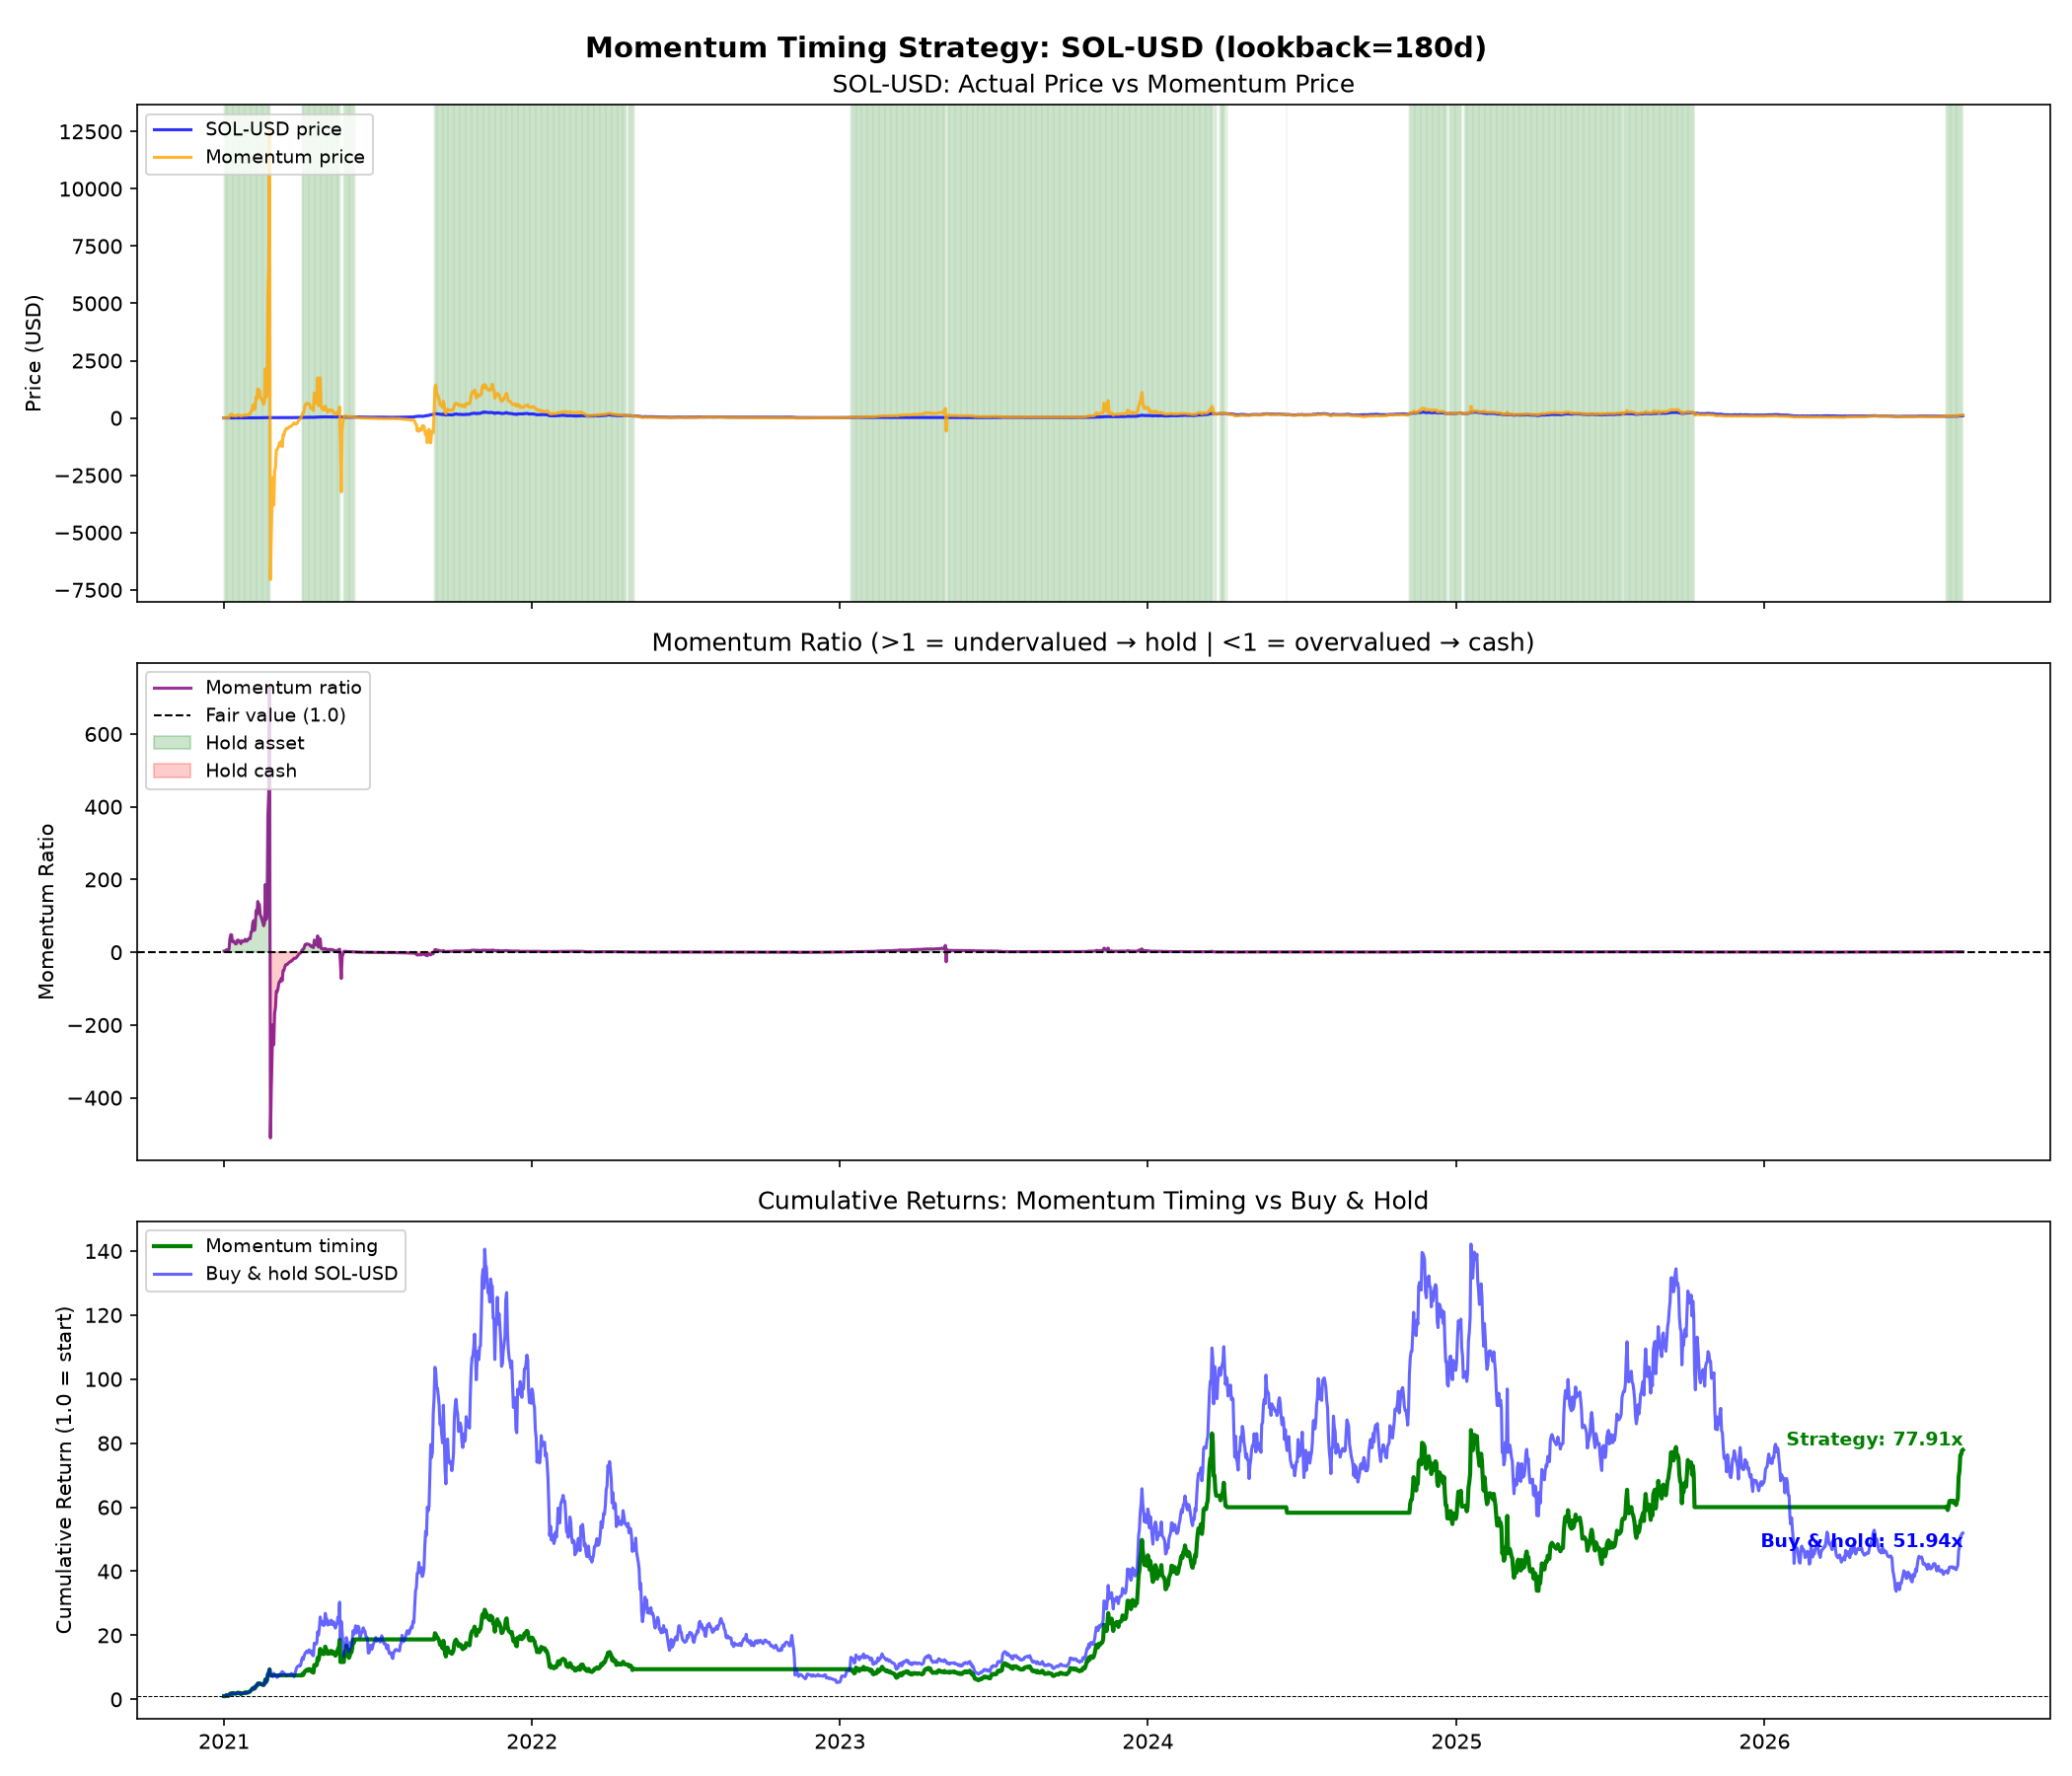
\includegraphics[width=\textwidth]{timing_SOLUSD.png}
    \caption{Solana: the model avoids the 2022 crash ($-96\%$) and
    catches the 2023--2025 recovery. Strategy returns 78x vs buy \&
    hold's 52x.}
\end{figure}

\section{Chart: BTC-USD (180-day lookback)}

\begin{figure}[H]
    \centering
    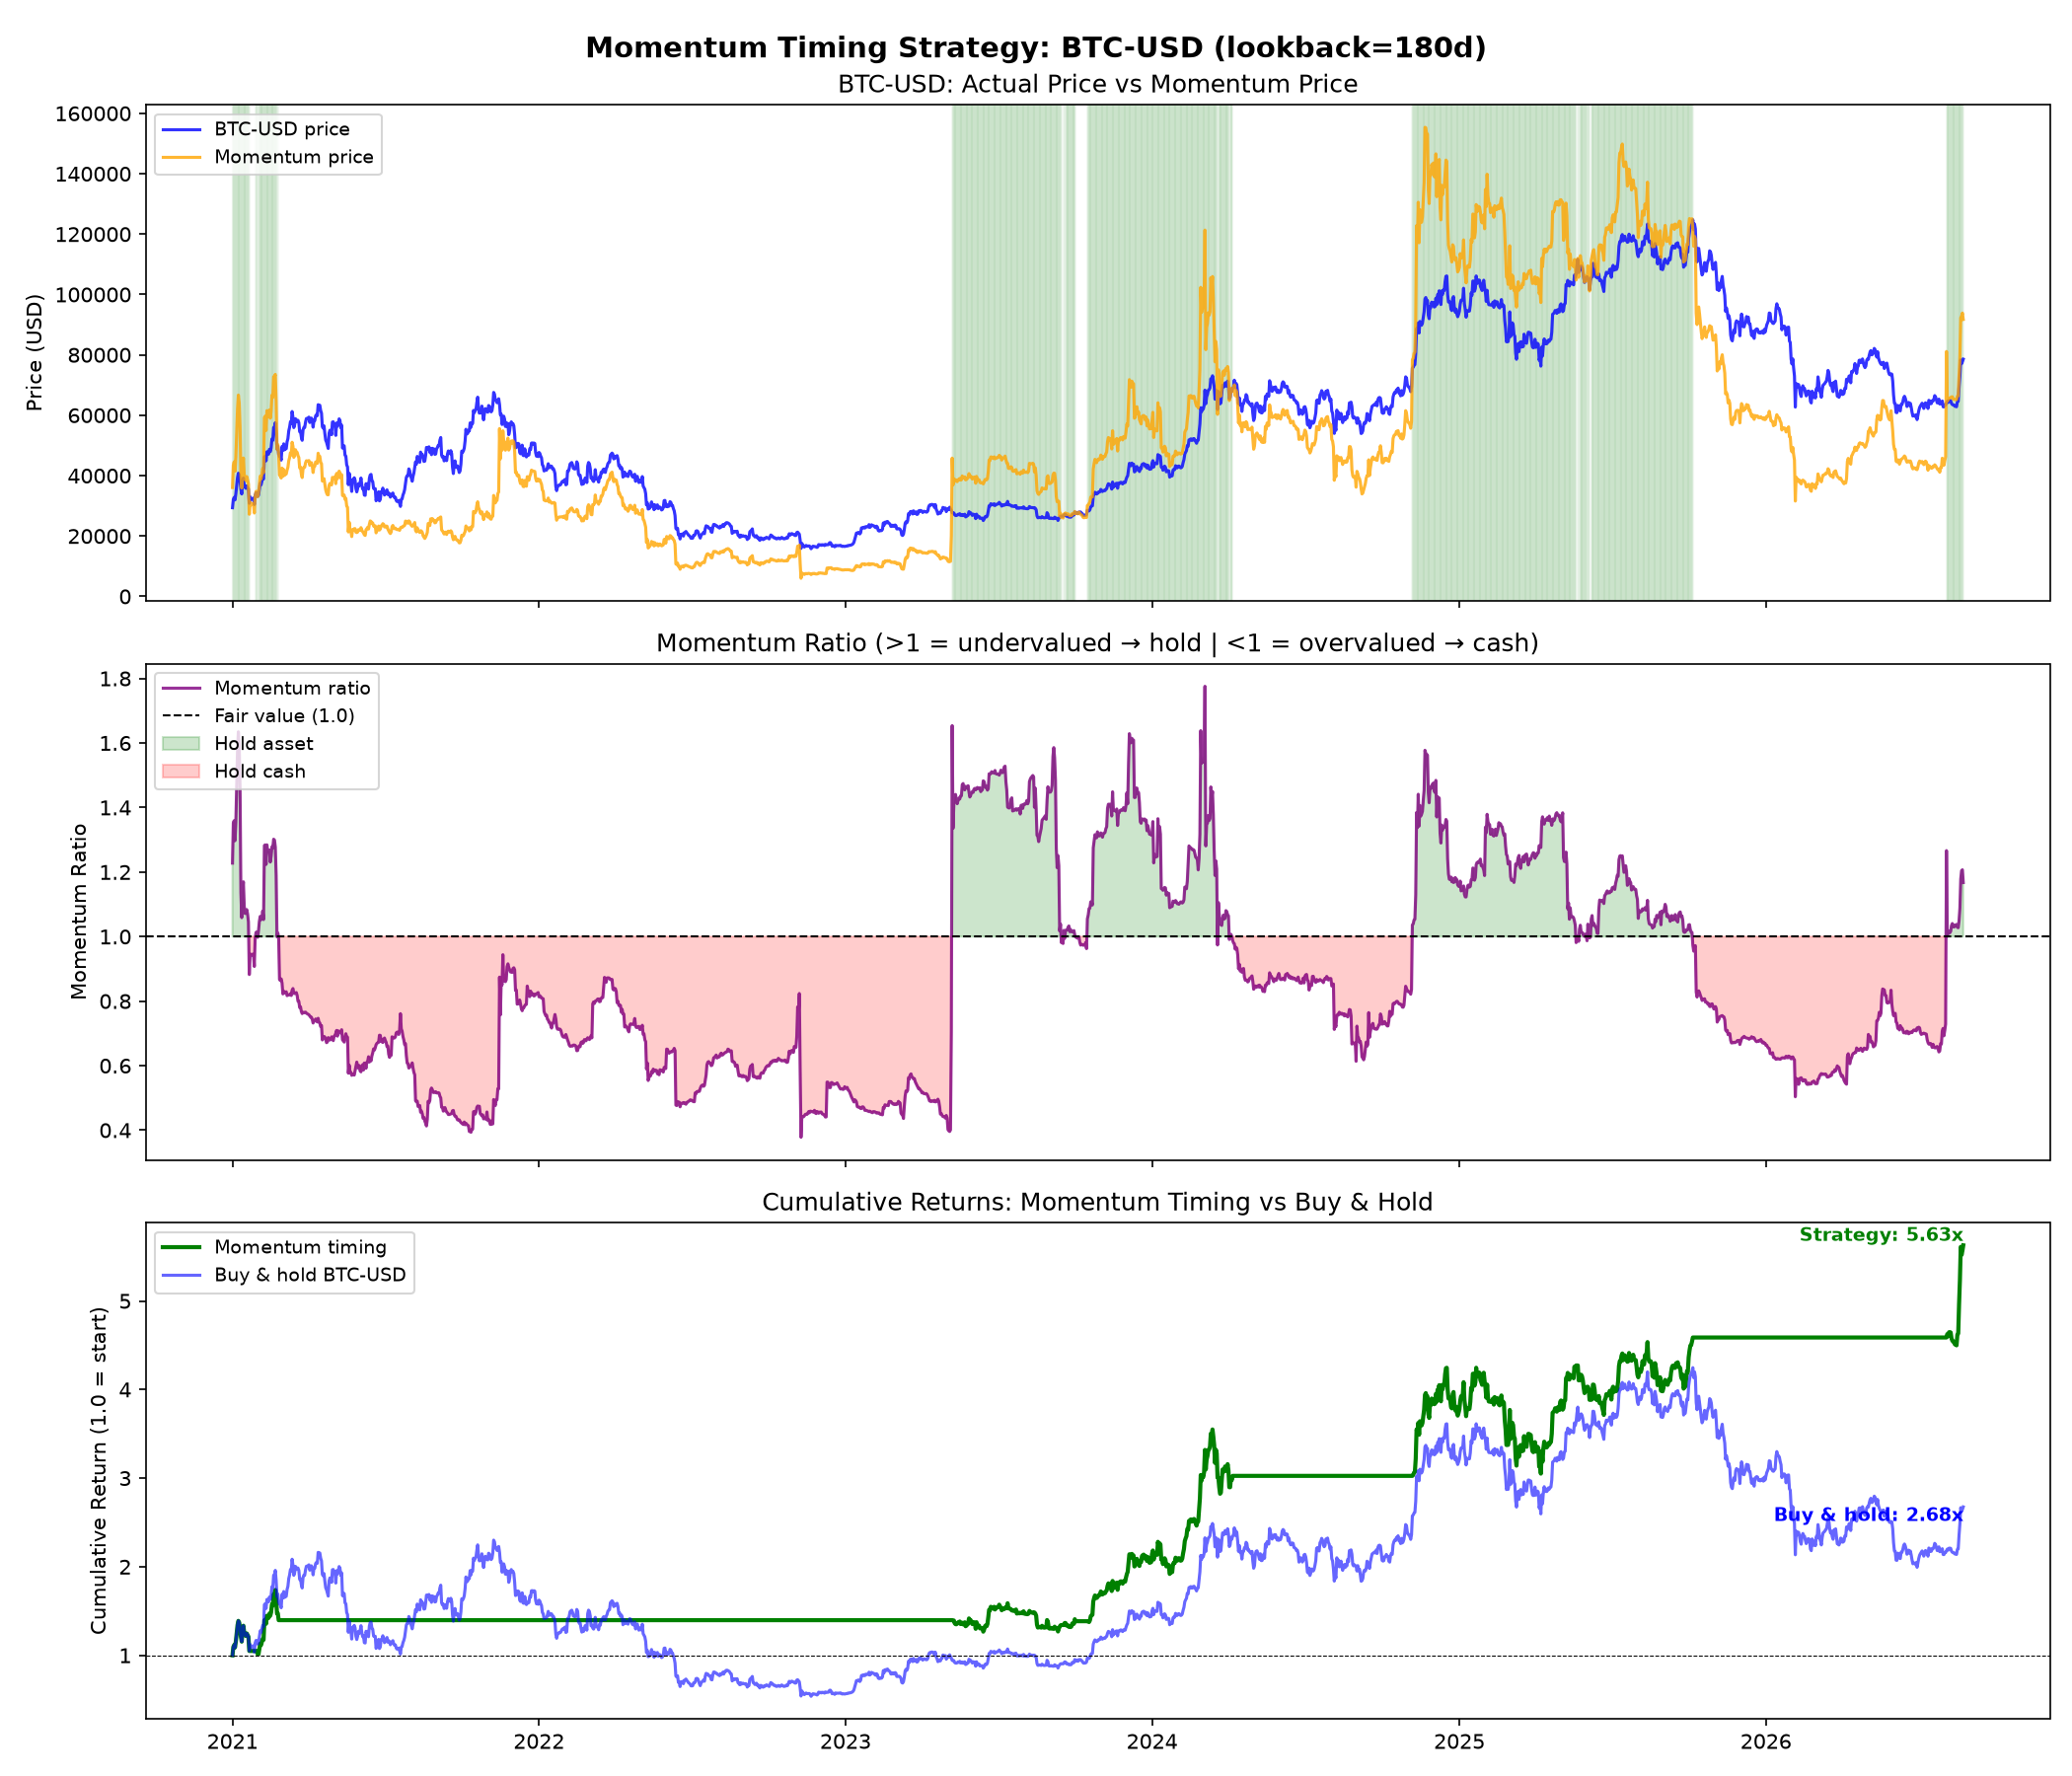
\includegraphics[width=\textwidth]{timing_BTCUSD.png}
    \caption{Top: BTC price (blue) vs momentum price (orange), with
    green shading when the strategy holds BTC. Middle: momentum ratio
    with hold/cash zones. Bottom: cumulative returns --- strategy
    (green, 5.63x) vs buy \& hold (blue, 2.68x).}
\end{figure}

Key observations:

\begin{enumerate}[leftmargin=2em]
    \item The strategy \textbf{exits before the 2022 crash} ---
          the momentum ratio drops below 1.0 as volume flows turn
          negative.
    \item It \textbf{re-enters during the 2023 accumulation},
          when volume flows turn positive while the price is still low.
    \item It \textbf{rides the 2024--2025 bull run} but exits during
          corrections, preserving gains.
\end{enumerate}

\section{BTC Lookback Sensitivity}

\begin{itemize}[leftmargin=2em]
    \item \textbf{90 days}: Too reactive. 22 trades, 45\% win rate.
          Whipsawed by noise. Average losses (-9.2\%) too large.
    \item \textbf{180 days}: The sweet spot. 16 trades, 62\% win rate.
          Captures major regime shifts without overtrading.
    \item \textbf{365 days}: Too slow. 10 trades, enters and exits
          late. Returns +132\% vs buy \& hold's +167\%.
\end{itemize}

\newpage

% ══════════════════════════════════════════════════════════════════
% PART III: PRECIOUS METALS
% ══════════════════════════════════════════════════════════════════

\part{Precious Metals}

\section{Gold (GC=F): 2010--2026}

\begin{figure}[H]
    \centering
    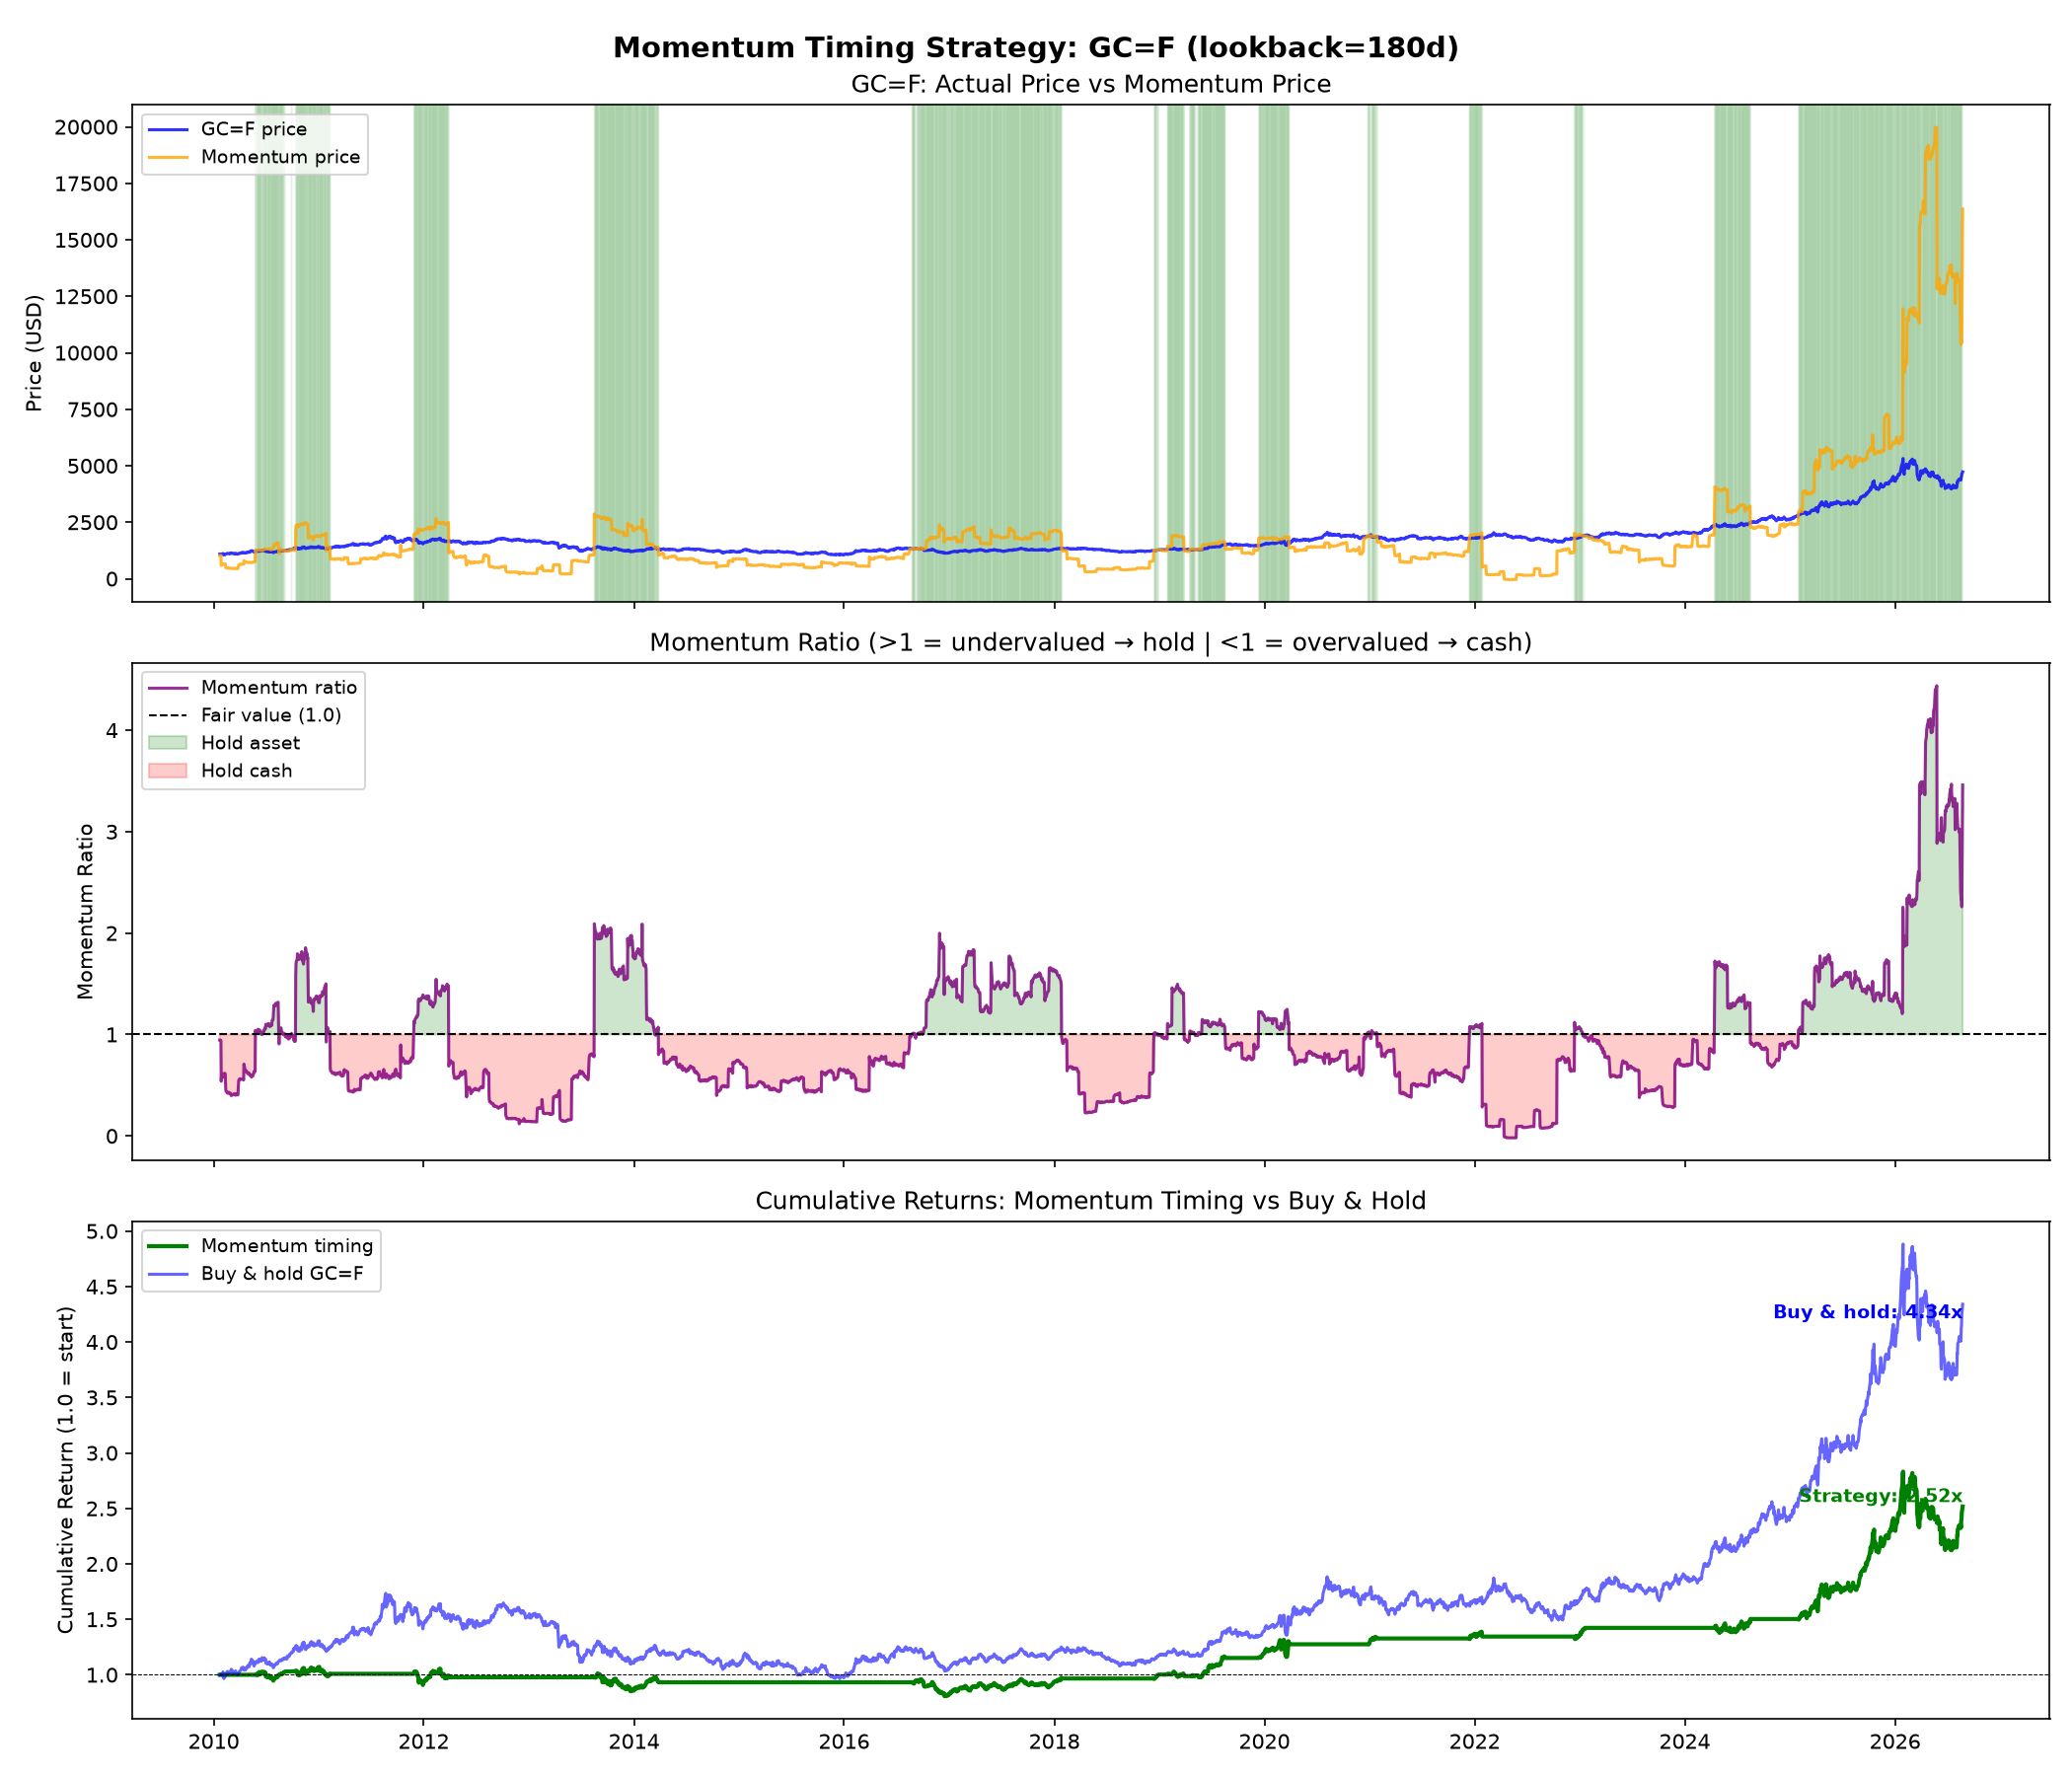
\includegraphics[width=\textwidth]{timing_gold.png}
    \caption{Gold: 16 years of momentum timing. The strategy captures
    rallies (2010--11, 2020--26) but gets whipsawed during the
    sideways years (2014--18).}
\end{figure}

\subsection{Results}

\vspace{0.5em}
\begin{tabular}{@{}lrrr@{}}
    \toprule
    \textbf{Metric} & \textbf{90-day} & \textbf{180-day} & \textbf{365-day} \\
    \midrule
    Strategy return    & $+114.5\%$ & $+151.7\%$ & $+131.6\%$ \\
    Buy \& hold return & $+323.0\%$ & $+334.1\%$ & $+316.5\%$ \\
    Alpha              & $-208.6\%$ & $-182.3\%$ & $-184.9\%$ \\
    Sharpe ratio       & $0.51$     & $0.66$     & $0.72$     \\
    Max drawdown       & $-29.3\%$  & $-25.1\%$  & $-25.1\%$  \\
    Buy \& hold DD     & $-44.4\%$  & $-44.4\%$  & $-44.4\%$  \\
    Trades             & 40         & 30         & 6          \\
    \bottomrule
\end{tabular}

\subsection{Recent Period: 2021--2026 Only}

\vspace{0.5em}
\begin{tabular}{@{}lr@{}}
    \toprule
    \textbf{Metric} & \textbf{180-day} \\
    \midrule
    Strategy return    & $+88.7\%$  \\
    Buy \& hold return & $+154.8\%$ \\
    Alpha              & $-66.2\%$  \\
    Sharpe ratio       & $1.03$     \\
    Max drawdown       & $-25.1\%$  \\
    Win rate           & 83\% (5/6) \\
    Avg win / loss     & $+16.4\%$ / $-0.7\%$ \quad (23:1 ratio) \\
    \bottomrule
\end{tabular}

\begin{resultbox}[Verdict: Gold --- Risk Management Only]{promising}
The strategy \textbf{does not beat buy \& hold on return}. Gold's long
sideways periods (2014--2018) create whipsaw losses that eat the gains
from catching rallies. However: max drawdown is \textbf{$-25.1\%$ vs
$-44.4\%$} (nearly halved), recent win rate is \textbf{83\%} with a
\textbf{23:1} win/loss asymmetry. Best used as a \textbf{risk
management} tool, not a return maximiser.
\end{resultbox}

\newpage

\section{Silver (SI=F): 2010--2026}

\begin{figure}[H]
    \centering
    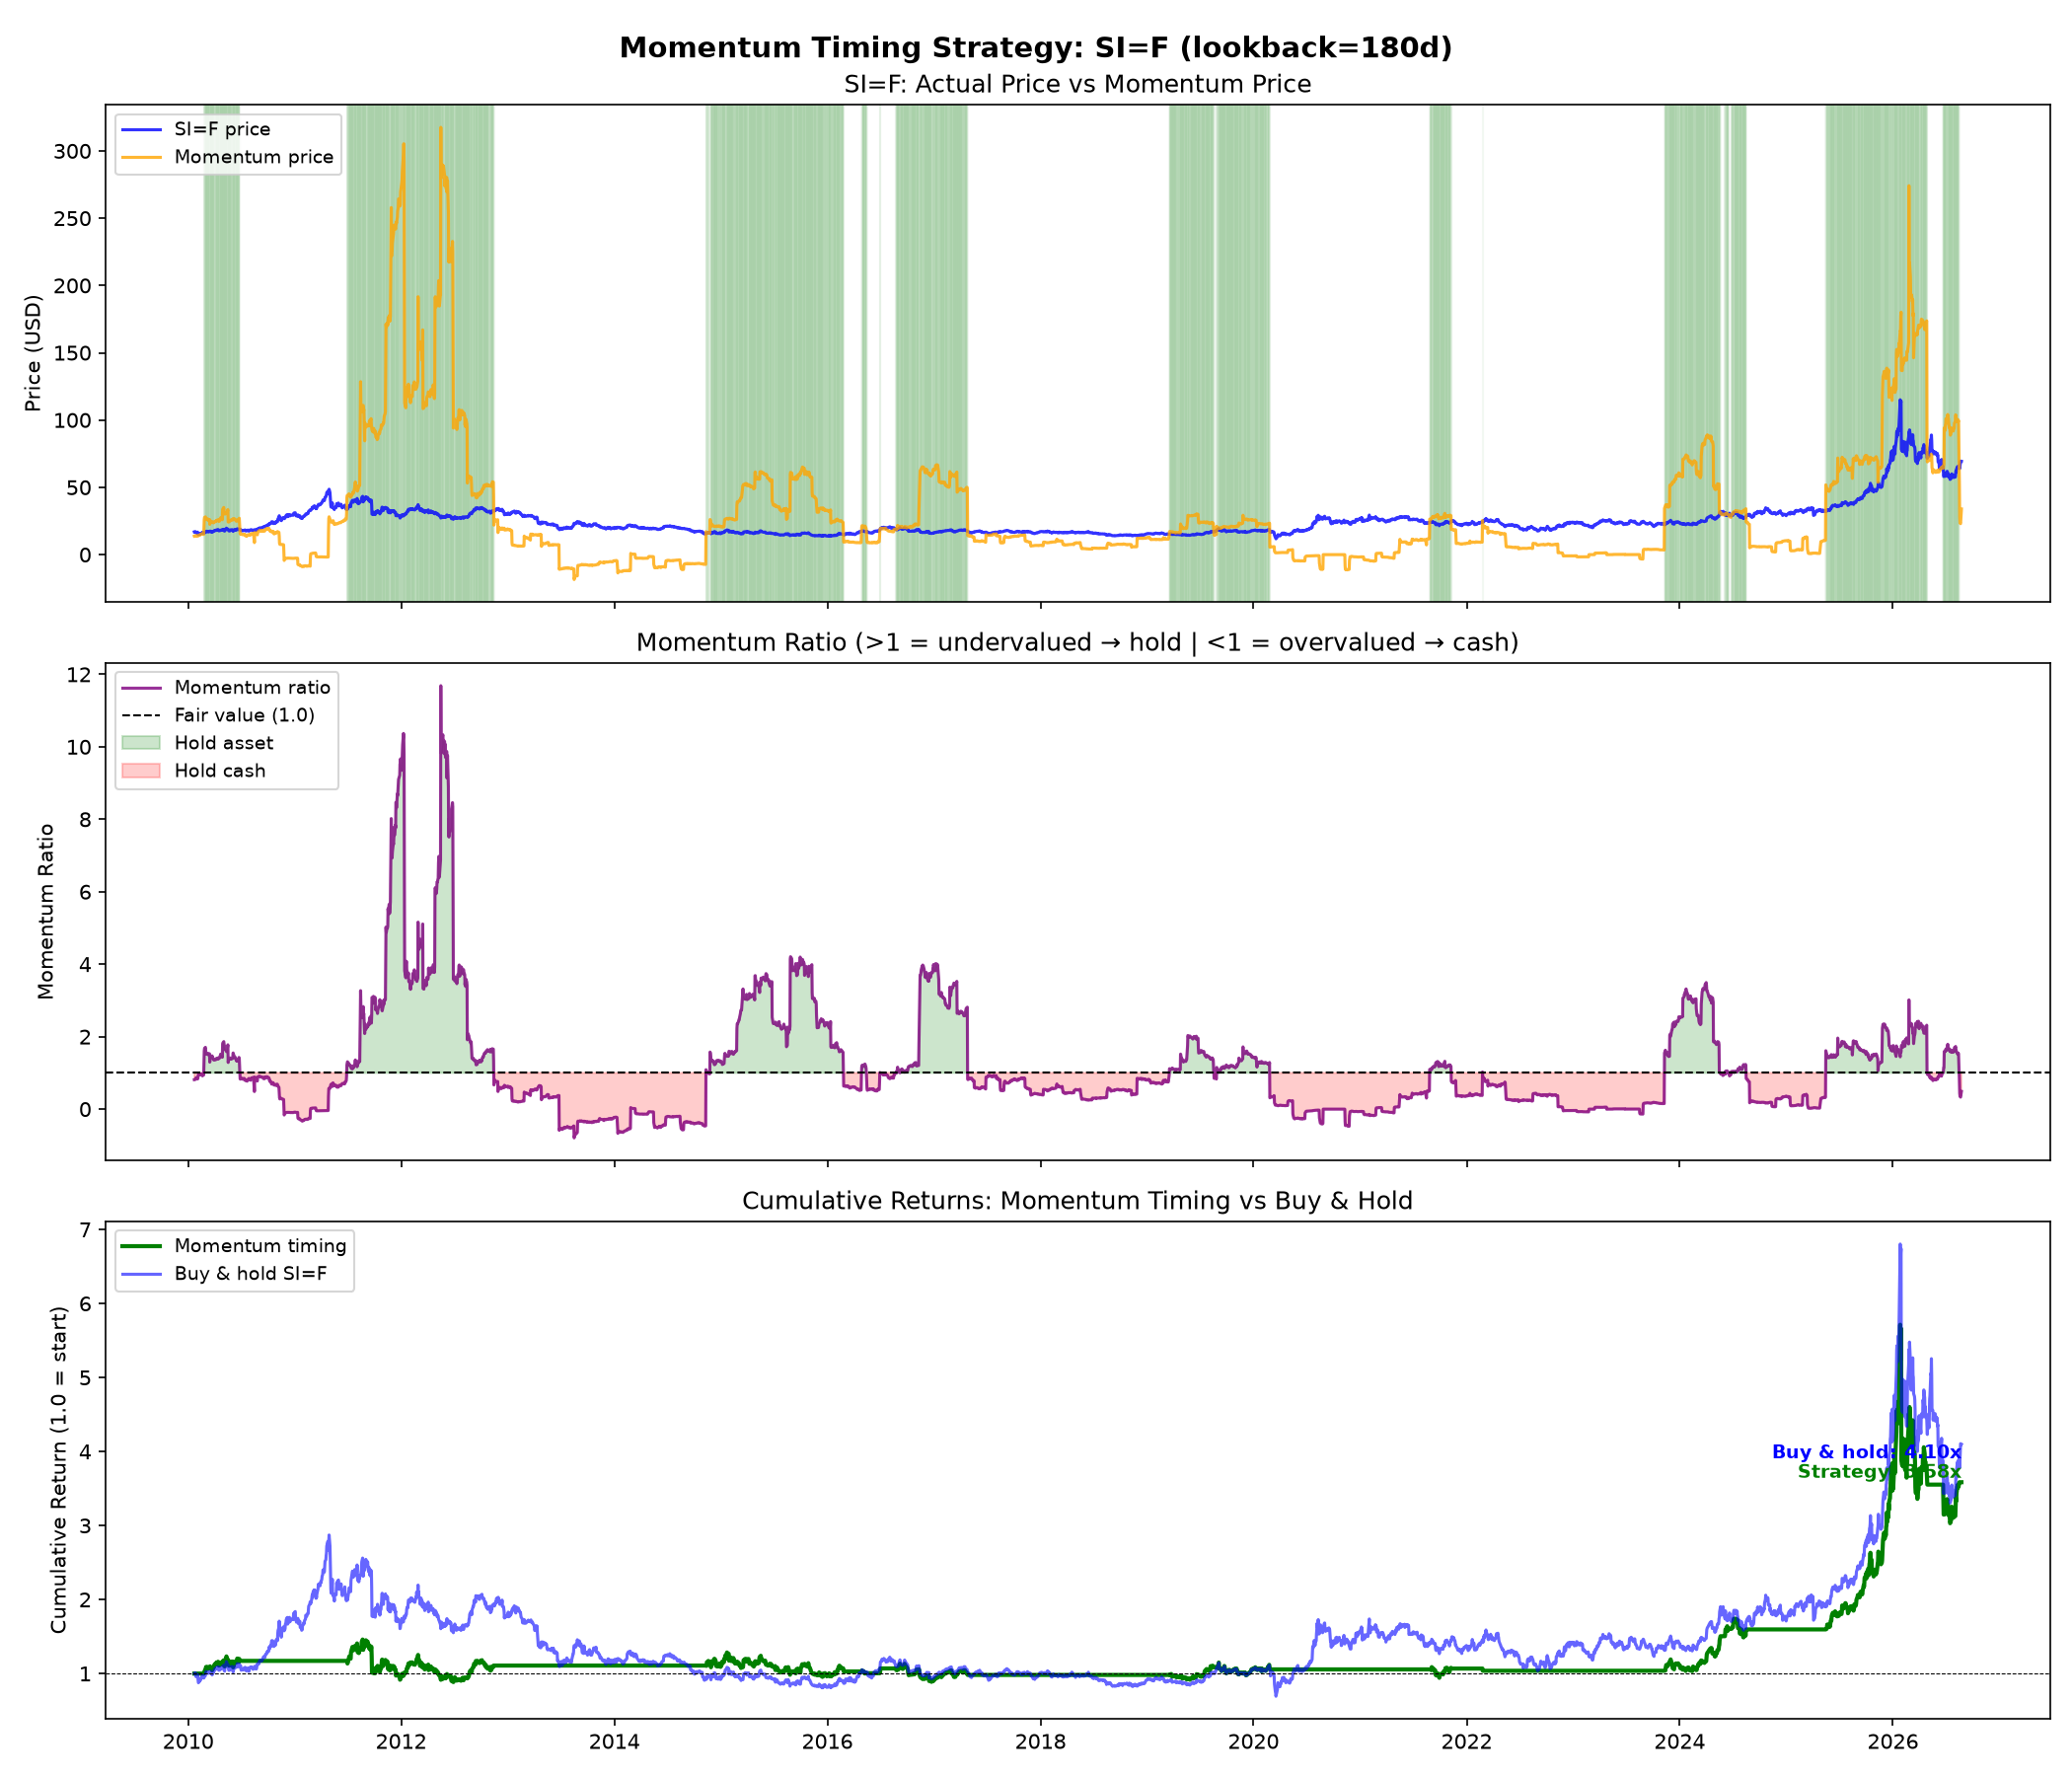
\includegraphics[width=\textwidth]{timing_silver.png}
    \caption{Silver: 16 years of momentum timing. The strategy avoids
    the catastrophic 2011--2015 crash (-72\%) and captures the
    2024--2026 rally.}
\end{figure}

\subsection{Results}

\vspace{0.5em}
\begin{tabular}{@{}lrrr@{}}
    \toprule
    \textbf{Metric} & \textbf{90-day} & \textbf{180-day} & \textbf{365-day} \\
    \midrule
    Strategy return    & $+90.0\%$  & $+258.5\%$ & $-12.5\%$  \\
    Buy \& hold return & $+297.6\%$ & $+309.9\%$ & $+291.2\%$ \\
    Alpha              & $-207.6\%$ & $-51.4\%$  & $-303.7\%$ \\
    Sharpe ratio       & $0.34$     & $0.54$     & $0.03$     \\
    Max drawdown       & $-63.9\%$  & $-46.9\%$  & $-41.0\%$  \\
    Buy \& hold DD     & $-75.8\%$  & $-75.8\%$  & $-75.8\%$  \\
    Trades             & 33         & 18         & 9          \\
    \bottomrule
\end{tabular}

\subsection{Recent Period: 2021--2026 Only}

\vspace{0.5em}
\begin{tabular}{@{}lr@{}}
    \toprule
    \textbf{Metric} & \textbf{180-day} \\
    \midrule
    Strategy return    & \textcolor{green}{\textbf{+239.3\%}} \\
    Buy \& hold return & $+171.7\%$ \\
    Alpha              & \textcolor{green}{\textbf{+67.6\%}} \\
    Sharpe ratio       & \textcolor{green}{\textbf{1.09}} \\
    Max drawdown       & $-46.9\%$  \\
    Win rate           & 88\% (7/8) \\
    Avg win / loss     & $+26.1\%$ / $-2.0\%$ \quad (13:1 ratio) \\
    \bottomrule
\end{tabular}

\begin{resultbox}[Verdict: Silver --- Promising]{promising}
Silver is the \textbf{most interesting} precious metal for this
strategy. Over 16 years: captures \textbf{83\% of buy \& hold return}
while reducing max drawdown from $-75.8\%$ to $-46.9\%$. Recent
5 years: \textbf{+67.6\% alpha}, Sharpe 1.09, \textbf{88\% win rate}.
Silver's high volatility gives the momentum signal something to work
with --- large moves that the pool model detects early.
\end{resultbox}

\newpage

% ══════════════════════════════════════════════════════════════════
% PART IV: FOREX
% ══════════════════════════════════════════════════════════════════

\part{Foreign Exchange}

\section{The Volume Problem}

Forex is the most liquid market in the world (\$7.5 trillion/day),
but it is traded \textbf{over the counter} --- there is no central
exchange. This means there is no consolidated volume tape. Yahoo
Finance reports \textbf{zero volume} for spot forex pairs like
EURUSD=X.

The bookmaker model depends on volume. No volume, no signal.

\subsection{The Fix: CME Futures}

Currency \textbf{futures} trade on the CME (Chicago Mercantile
Exchange) and \emph{do} report volume. We use the CME tickers:

\vspace{0.5em}
\begin{tabular}{@{}llr@{}}
    \toprule
    \textbf{Ticker} & \textbf{Currency} & \textbf{Typical volume} \\
    \midrule
    6E=F & Euro (EUR/USD)          & 170--1,300 contracts/day \\
    6S=F & Swiss Franc (CHF/USD)   & 13,000--26,000 \\
    6J=F & Japanese Yen (JPY/USD)  & 600--1,300 \\
    6B=F & British Pound (GBP/USD) & 30--530 \\
    6A=F & Australian Dollar (AUD/USD) & 40--240 \\
    6C=F & Canadian Dollar (CAD/USD)   & 8--280 \\
    \bottomrule
\end{tabular}

\vspace{0.5em}
\textbf{Caveat:} These volumes are from yfinance and appear to be
only a fraction of actual CME volumes (which are typically 100x
higher). The signals may improve with a proper futures data provider.

\section{Results: All Six Pairs (2021--2026)}

All results using 180-day lookback:

\vspace{0.5em}
\begin{tabular}{@{}lrrrrrr@{}}
    \toprule
    & \textbf{CHF} & \textbf{EUR} & \textbf{AUD}
    & \textbf{GBP} & \textbf{CAD} & \textbf{JPY} \\
    \midrule
    Strategy return
        & $+11.8\%$ & $+6.5\%$ & $+2.8\%$
        & $+2.5\%$ & $-4.2\%$ & $-23.0\%$ \\
    Buy \& hold
        & $+10.5\%$ & $-4.1\%$ & $-7.3\%$
        & $-0.3\%$ & $-7.9\%$ & $-34.7\%$ \\
    Alpha
        & $+1.2\%$ & \textcolor{green}{\textbf{+10.6\%}} & $+10.1\%$
        & $+2.9\%$ & $+3.7\%$ & $+11.7\%$ \\
    \midrule
    Sharpe
        & $0.36$ & $0.30$ & $0.13$
        & $0.14$ & $-0.27$ & $-0.70$ \\
    Max DD (strat)
        & $-9.3\%$ & $-7.5\%$ & $-12.7\%$
        & $-9.5\%$ & $-9.2\%$ & $-25.5\%$ \\
    Max DD (hold)
        & $-12.2\%$ & $-21.6\%$ & $-24.9\%$
        & $-24.8\%$ & $-17.4\%$ & $-36.7\%$ \\
    \midrule
    Days in asset
        & 70\% & 53\% & 43\%
        & 49\% & 39\% & 55\% \\
    Trades
        & 12 & 49 & 26
        & 14 & 21 & 7 \\
    Win rate
        & 33\% & 55\% & 42\%
        & 29\% & 29\% & 14\% \\
    \bottomrule
\end{tabular}

\section{Chart: EUR Futures (6E=F, 180-day lookback)}

\begin{figure}[H]
    \centering
    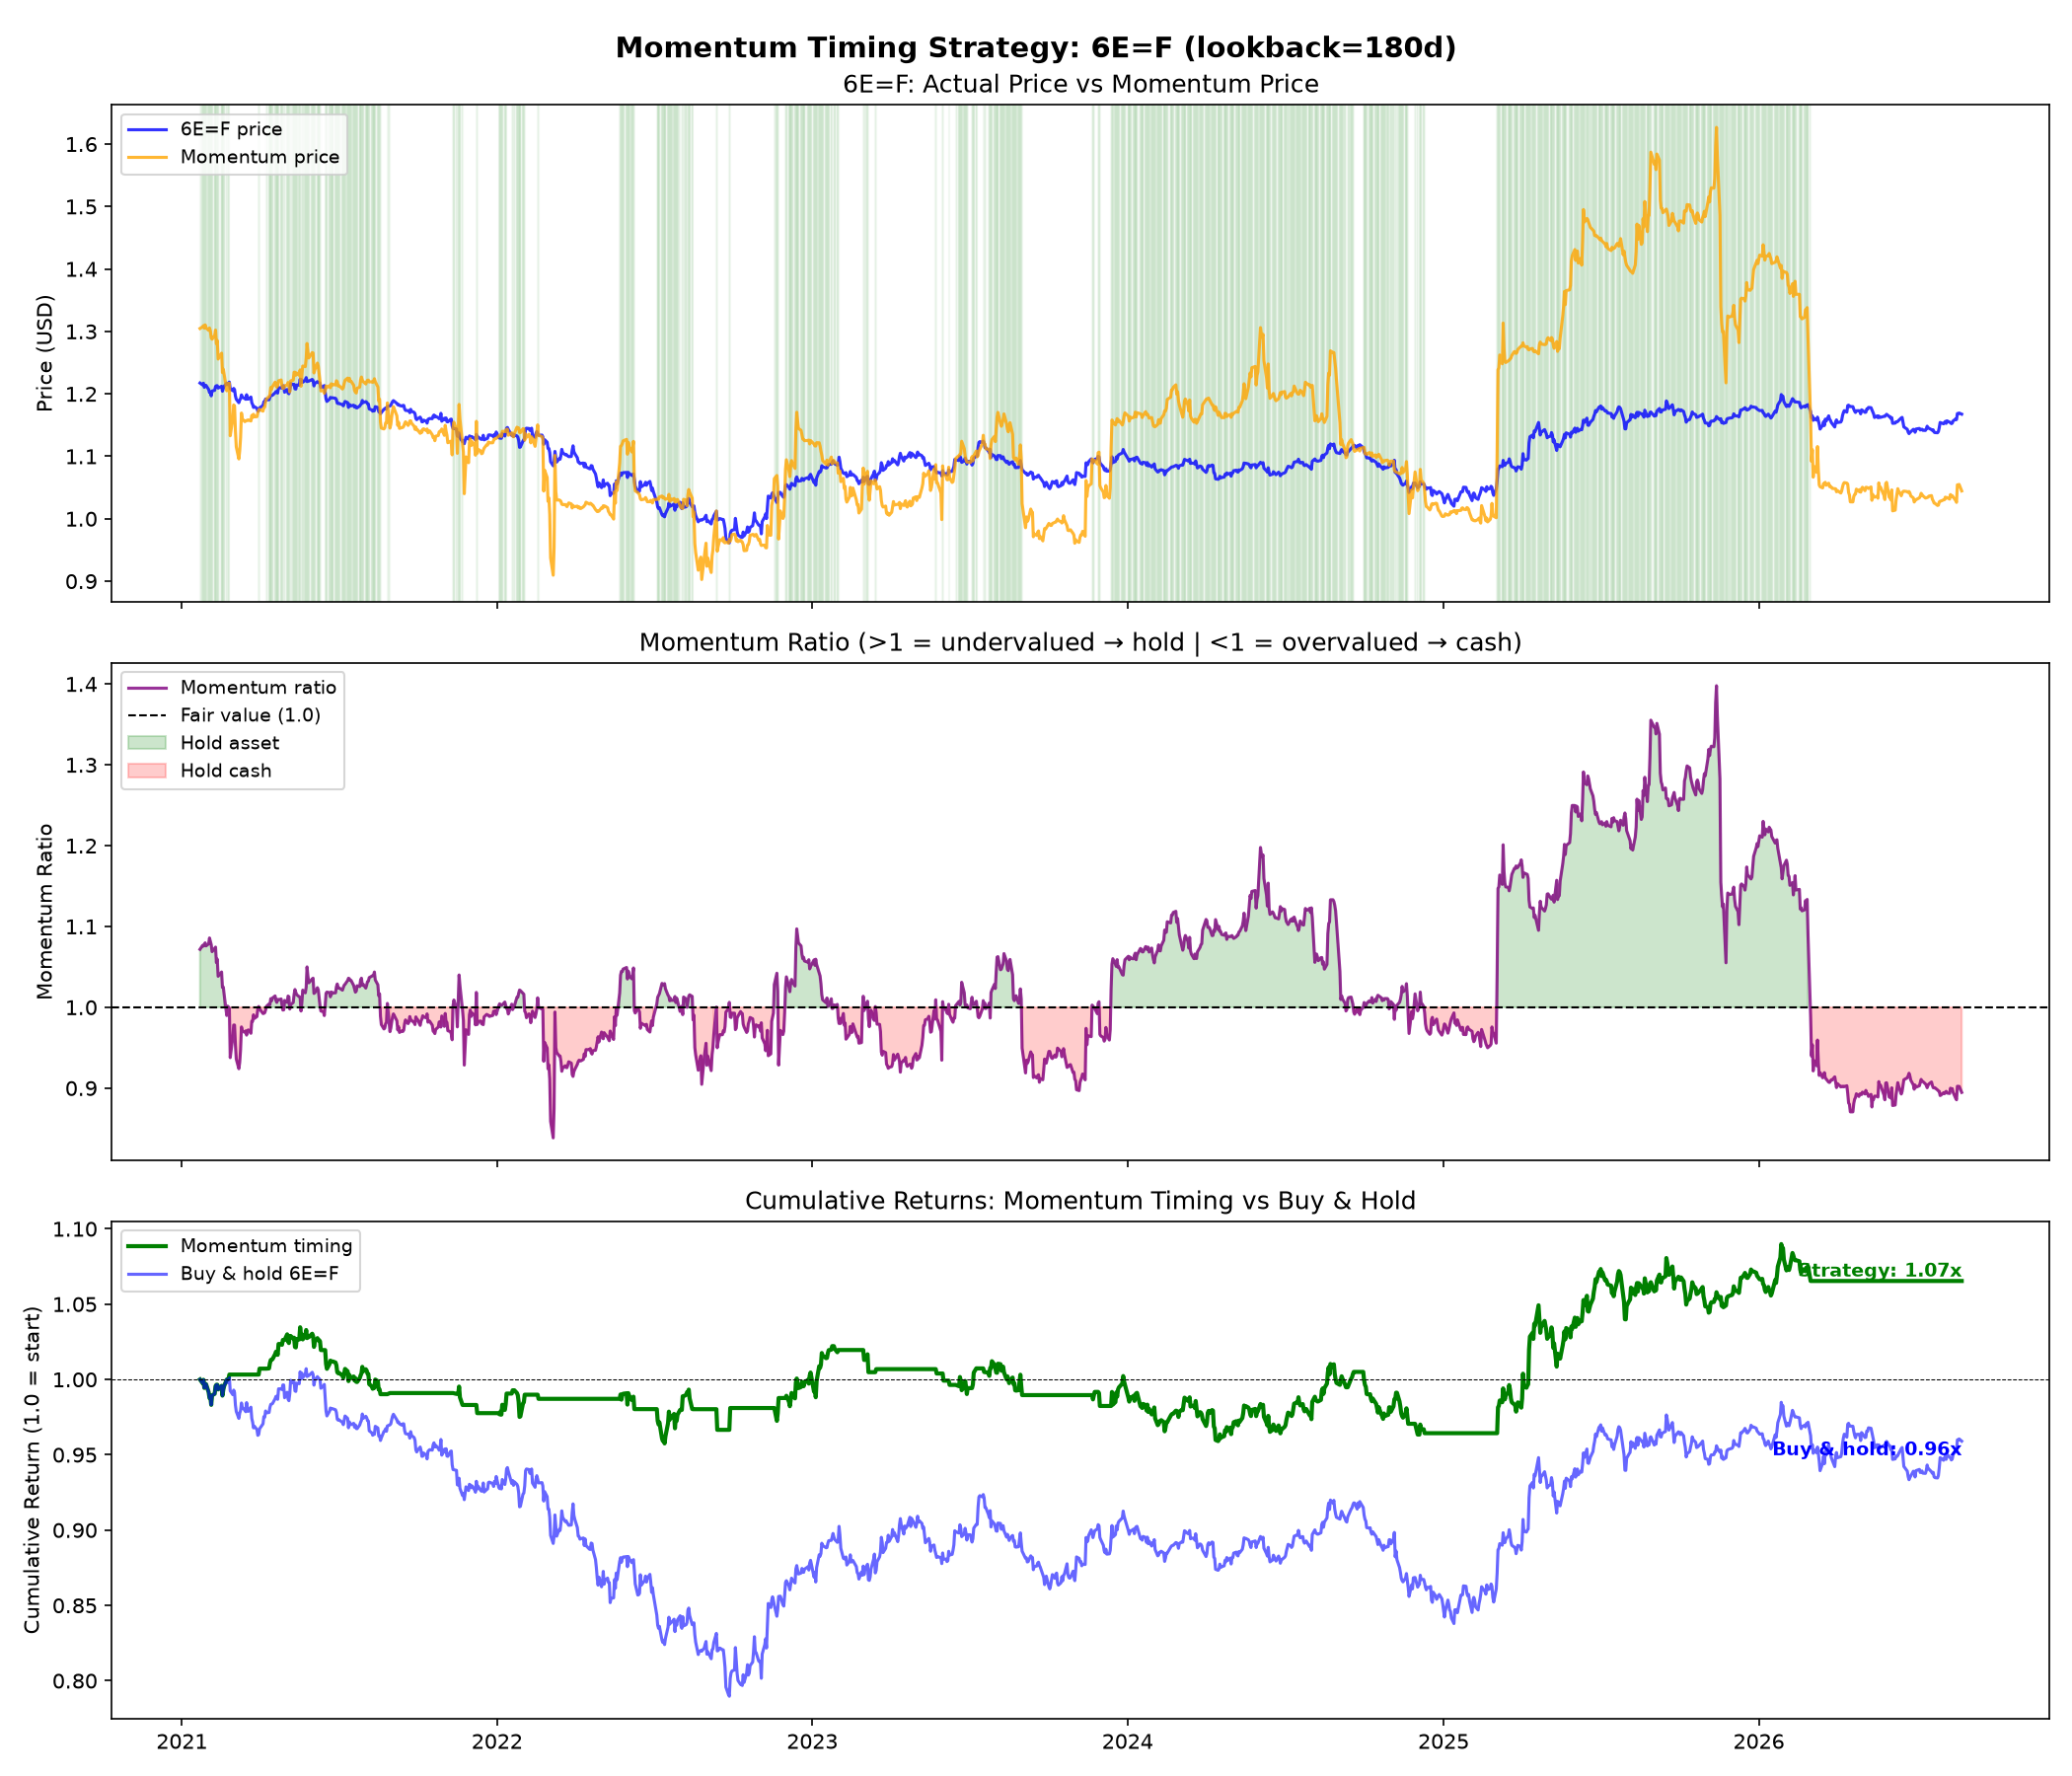
\includegraphics[width=\textwidth]{timing_6E=F.png}
    \caption{Euro futures: the model avoids the 2022 dollar strength
    rally (EUR fell 21\%) and re-enters for the 2023 recovery. Max
    drawdown cut from -21.6\% to -7.5\%.}
\end{figure}

\section{Verdict: Forex}

\textbf{Every pair has positive alpha.} The model consistently beats
buy \& hold, even when both lose money. But the story is very
different from crypto:

\begin{enumerate}[leftmargin=2em]
    \item \textbf{Drawdown reduction is excellent.} GBP drawdown cut
          from -24.8\% to -9.5\%. EUR from -21.6\% to -7.5\%. The
          model does what it does best --- getting you out before the
          worst of a move.

    \item \textbf{But returns are tiny.} FX pairs move 5--25\% over
          5 years. Compare that to Bitcoin's 167\% or silver's 310\%.
          The bookmaker model can't generate meaningful returns on
          assets that don't move much.

    \item \textbf{Volume data is suspect.} The yfinance CME volumes
          are a small fraction of actual trading volume. With proper
          data (from a futures broker or CME direct), the signal
          quality could improve substantially.

    \item \textbf{Win rates are poor.} Most pairs are below 50\%.
          The model gets whipsawed by the tight, mean-reverting
          ranges that characterise FX. Only EUR (55\%) is above
          coin-flip odds.

    \item \textbf{JPY is instructive.} Worst absolute return
          ($-23\%$) but best alpha ($+11.7\%$). The yen's secular
          decline since 2021 is so strong that even the model can't
          fight it --- but it avoids the worst of it.
\end{enumerate}

\begin{resultbox}[Verdict: Forex --- Risk Overlay Only]{neutral}
Forex momentum timing is a \textbf{risk management overlay}, not a
return generator. If you want FX exposure, EUR futures (6E=F) has the
cleanest signal. But for \emph{making money}, stick to crypto and
commodities.
\end{resultbox}

\newpage

% ══════════════════════════════════════════════════════════════════
% PART V: ENERGY COMMODITIES
% ══════════════════════════════════════════════════════════════════

\part{Energy Commodities}

Energy commodities are the most volatile traditional assets in the
world. Crude oil swings 50--80\% in a year; natural gas can double
or halve in months. If the bookmaker model needs volatility, energy
is the test.

\section{Crude Oil (CL=F): 2021--2026}

\begin{figure}[H]
    \centering
    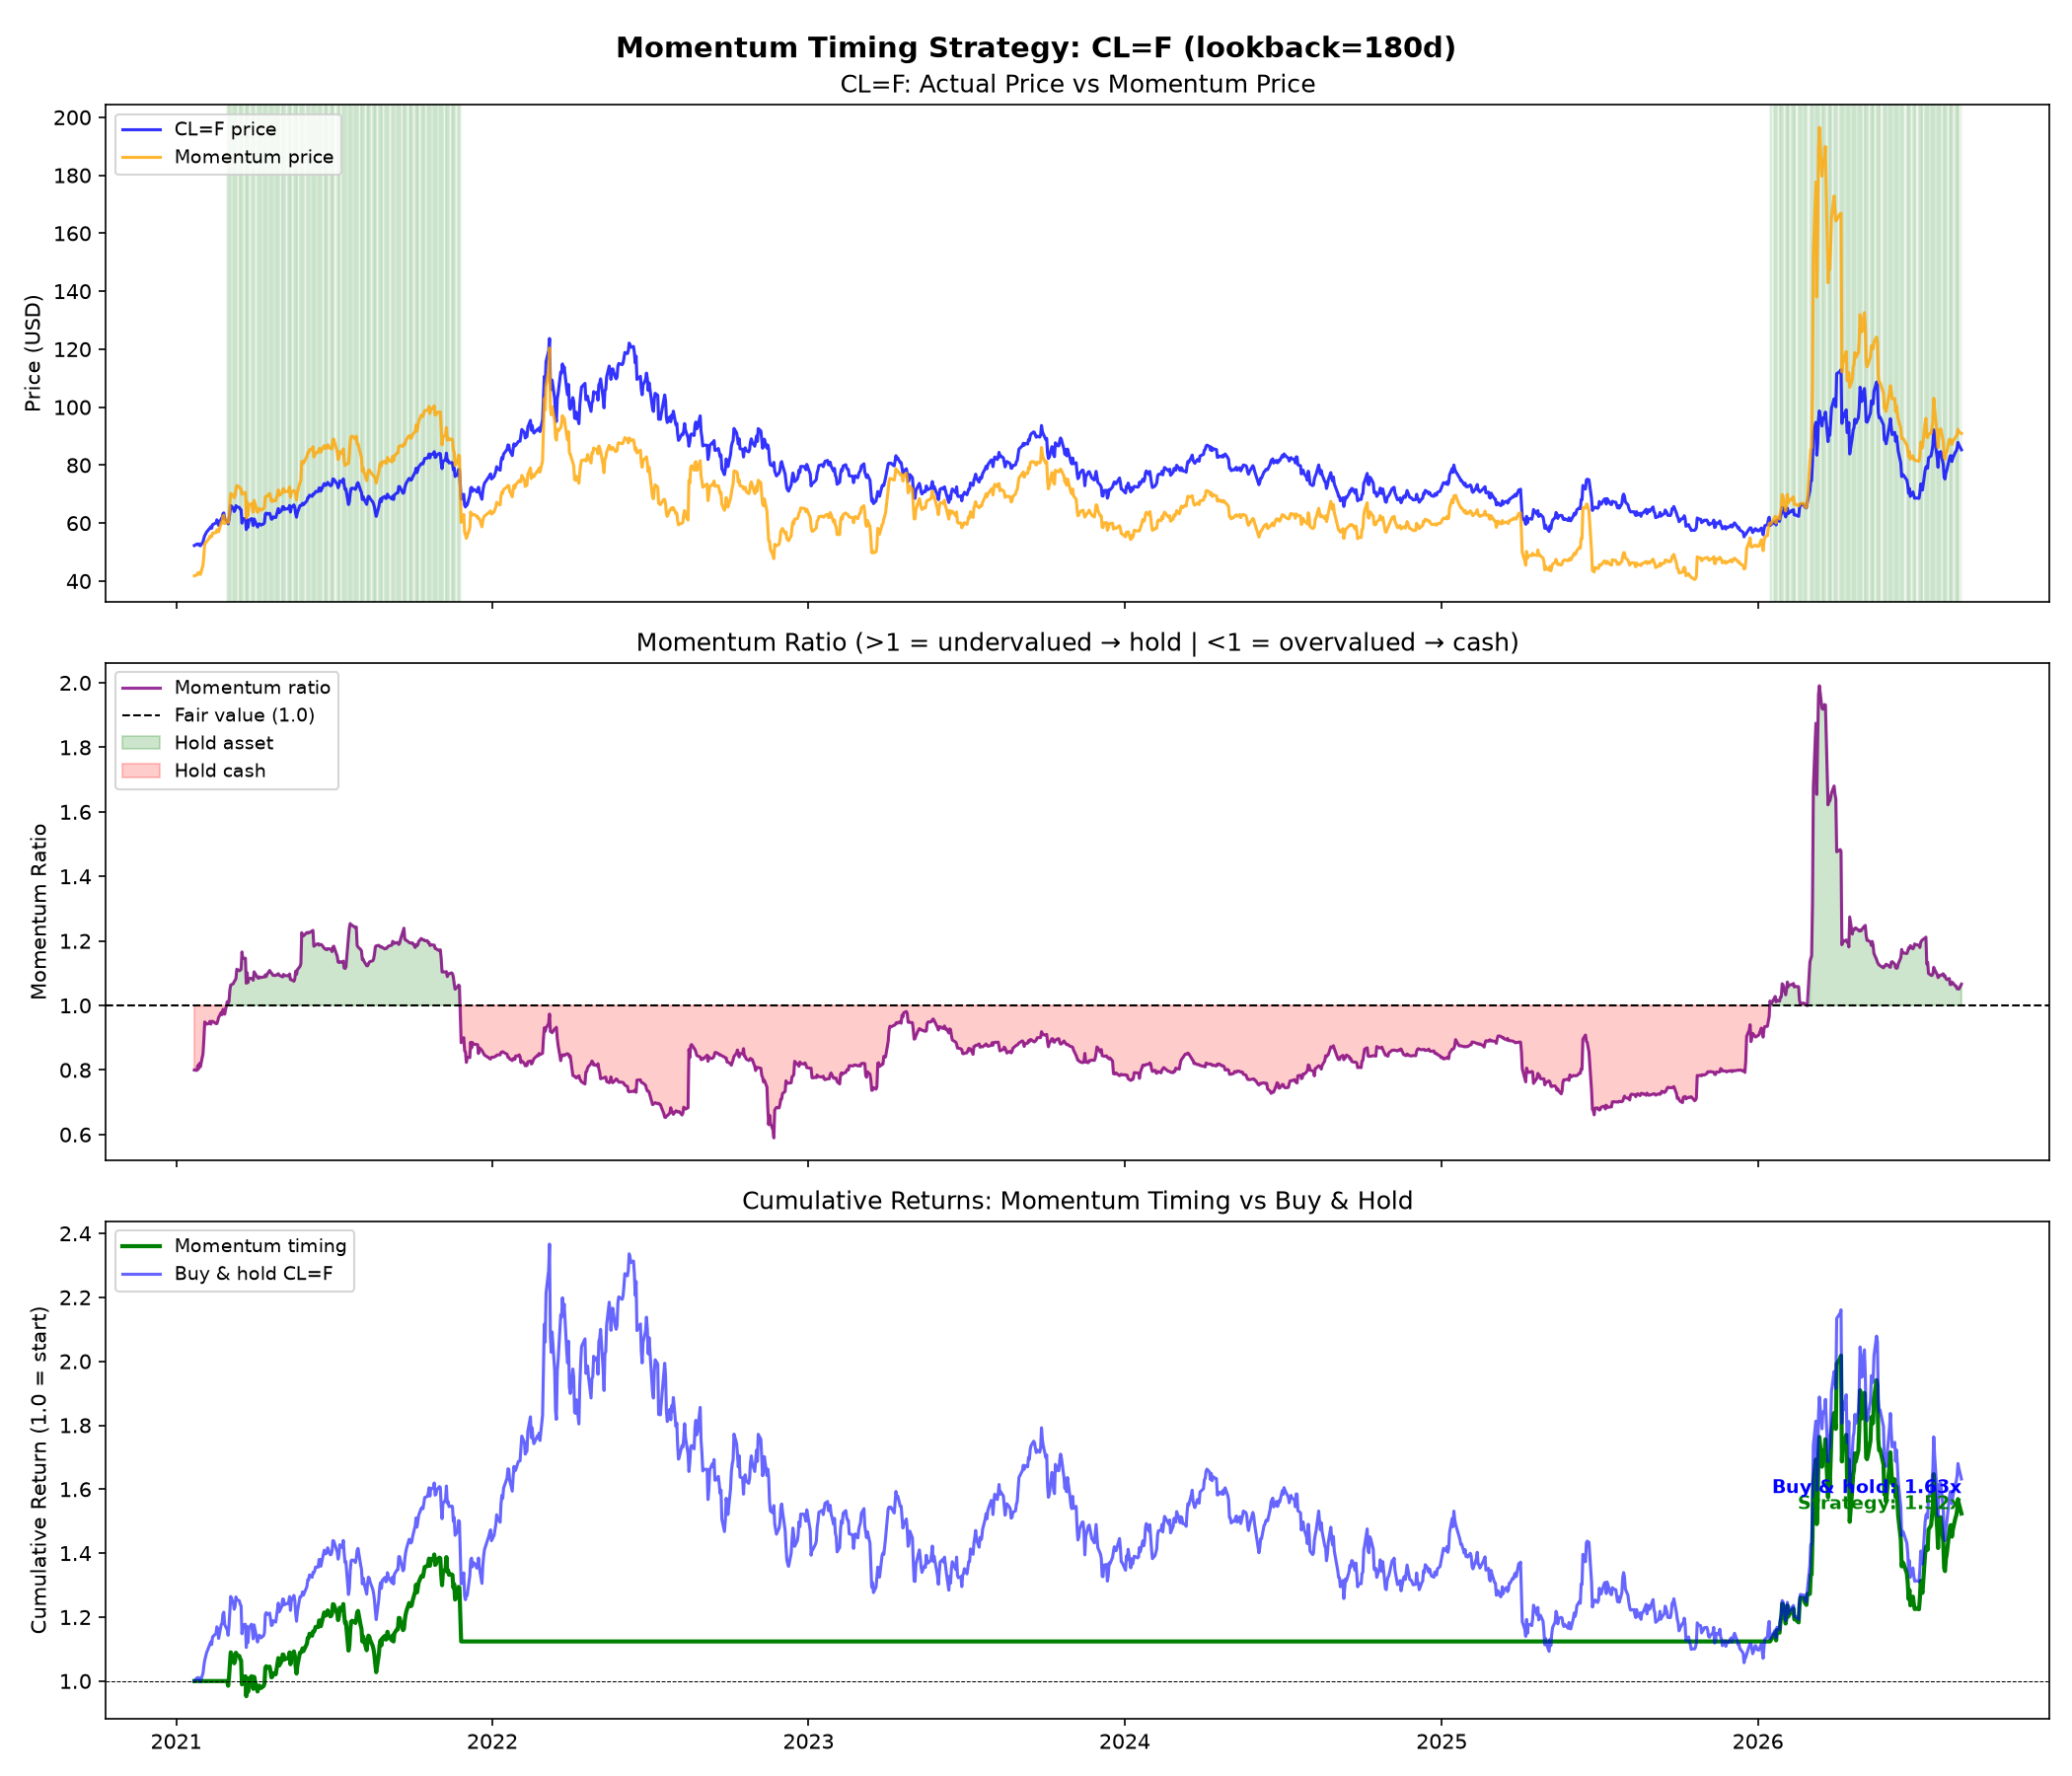
\includegraphics[width=\textwidth]{timing_CL=F.png}
    \caption{Crude oil: the model captures the 2021--2022 post-COVID
    rally and exits before the 2023 decline. Only 3 trades in 5 years
    at the 180-day lookback.}
\end{figure}

\subsection{Results}

\vspace{0.5em}
\begin{tabular}{@{}lrrr@{}}
    \toprule
    \textbf{Metric} & \textbf{90-day} & \textbf{180-day} & \textbf{365-day} \\
    \midrule
    Strategy return    & $+110.6\%$ & $+52.4\%$  & $+42.0\%$  \\
    Buy \& hold return & $+79.1\%$  & $+63.2\%$  & $+34.6\%$  \\
    Alpha              & \textcolor{green}{\textbf{+31.5\%}} & $-10.8\%$ & $+7.4\%$ \\
    Sharpe ratio       & $0.81$     & $0.51$     & $0.52$     \\
    Max drawdown       & $-34.3\%$  & $-39.3\%$  & $-23.2\%$  \\
    Buy \& hold DD     & $-55.3\%$  & $-55.3\%$  & $-55.3\%$  \\
    Trades             & 13         & 3          & 5          \\
    Win rate           & 62\%       & 100\%      & 80\%       \\
    Avg win            & $+16.1\%$  & $+17.1\%$  & $+14.0\%$  \\
    Avg loss           & $-4.6\%$   & ---        & $-17.4\%$  \\
    \bottomrule
\end{tabular}

\begin{resultbox}[Verdict: Crude Oil --- Risk Management]{promising}
Crude oil breaks the 180-day rule. The \textbf{90-day lookback}
produces the best result (+31.5\% alpha), while 180-day has negative
alpha. Oil markets move on geopolitical shocks and OPEC decisions that
play out over weeks, not months. All three lookbacks cut max drawdown
from $-55\%$ to $-23$--$39\%$. Best used as a \textbf{risk management
overlay} with 90-day lookback.
\end{resultbox}

\section{Natural Gas (NG=F): 2021--2026}

\begin{figure}[H]
    \centering
    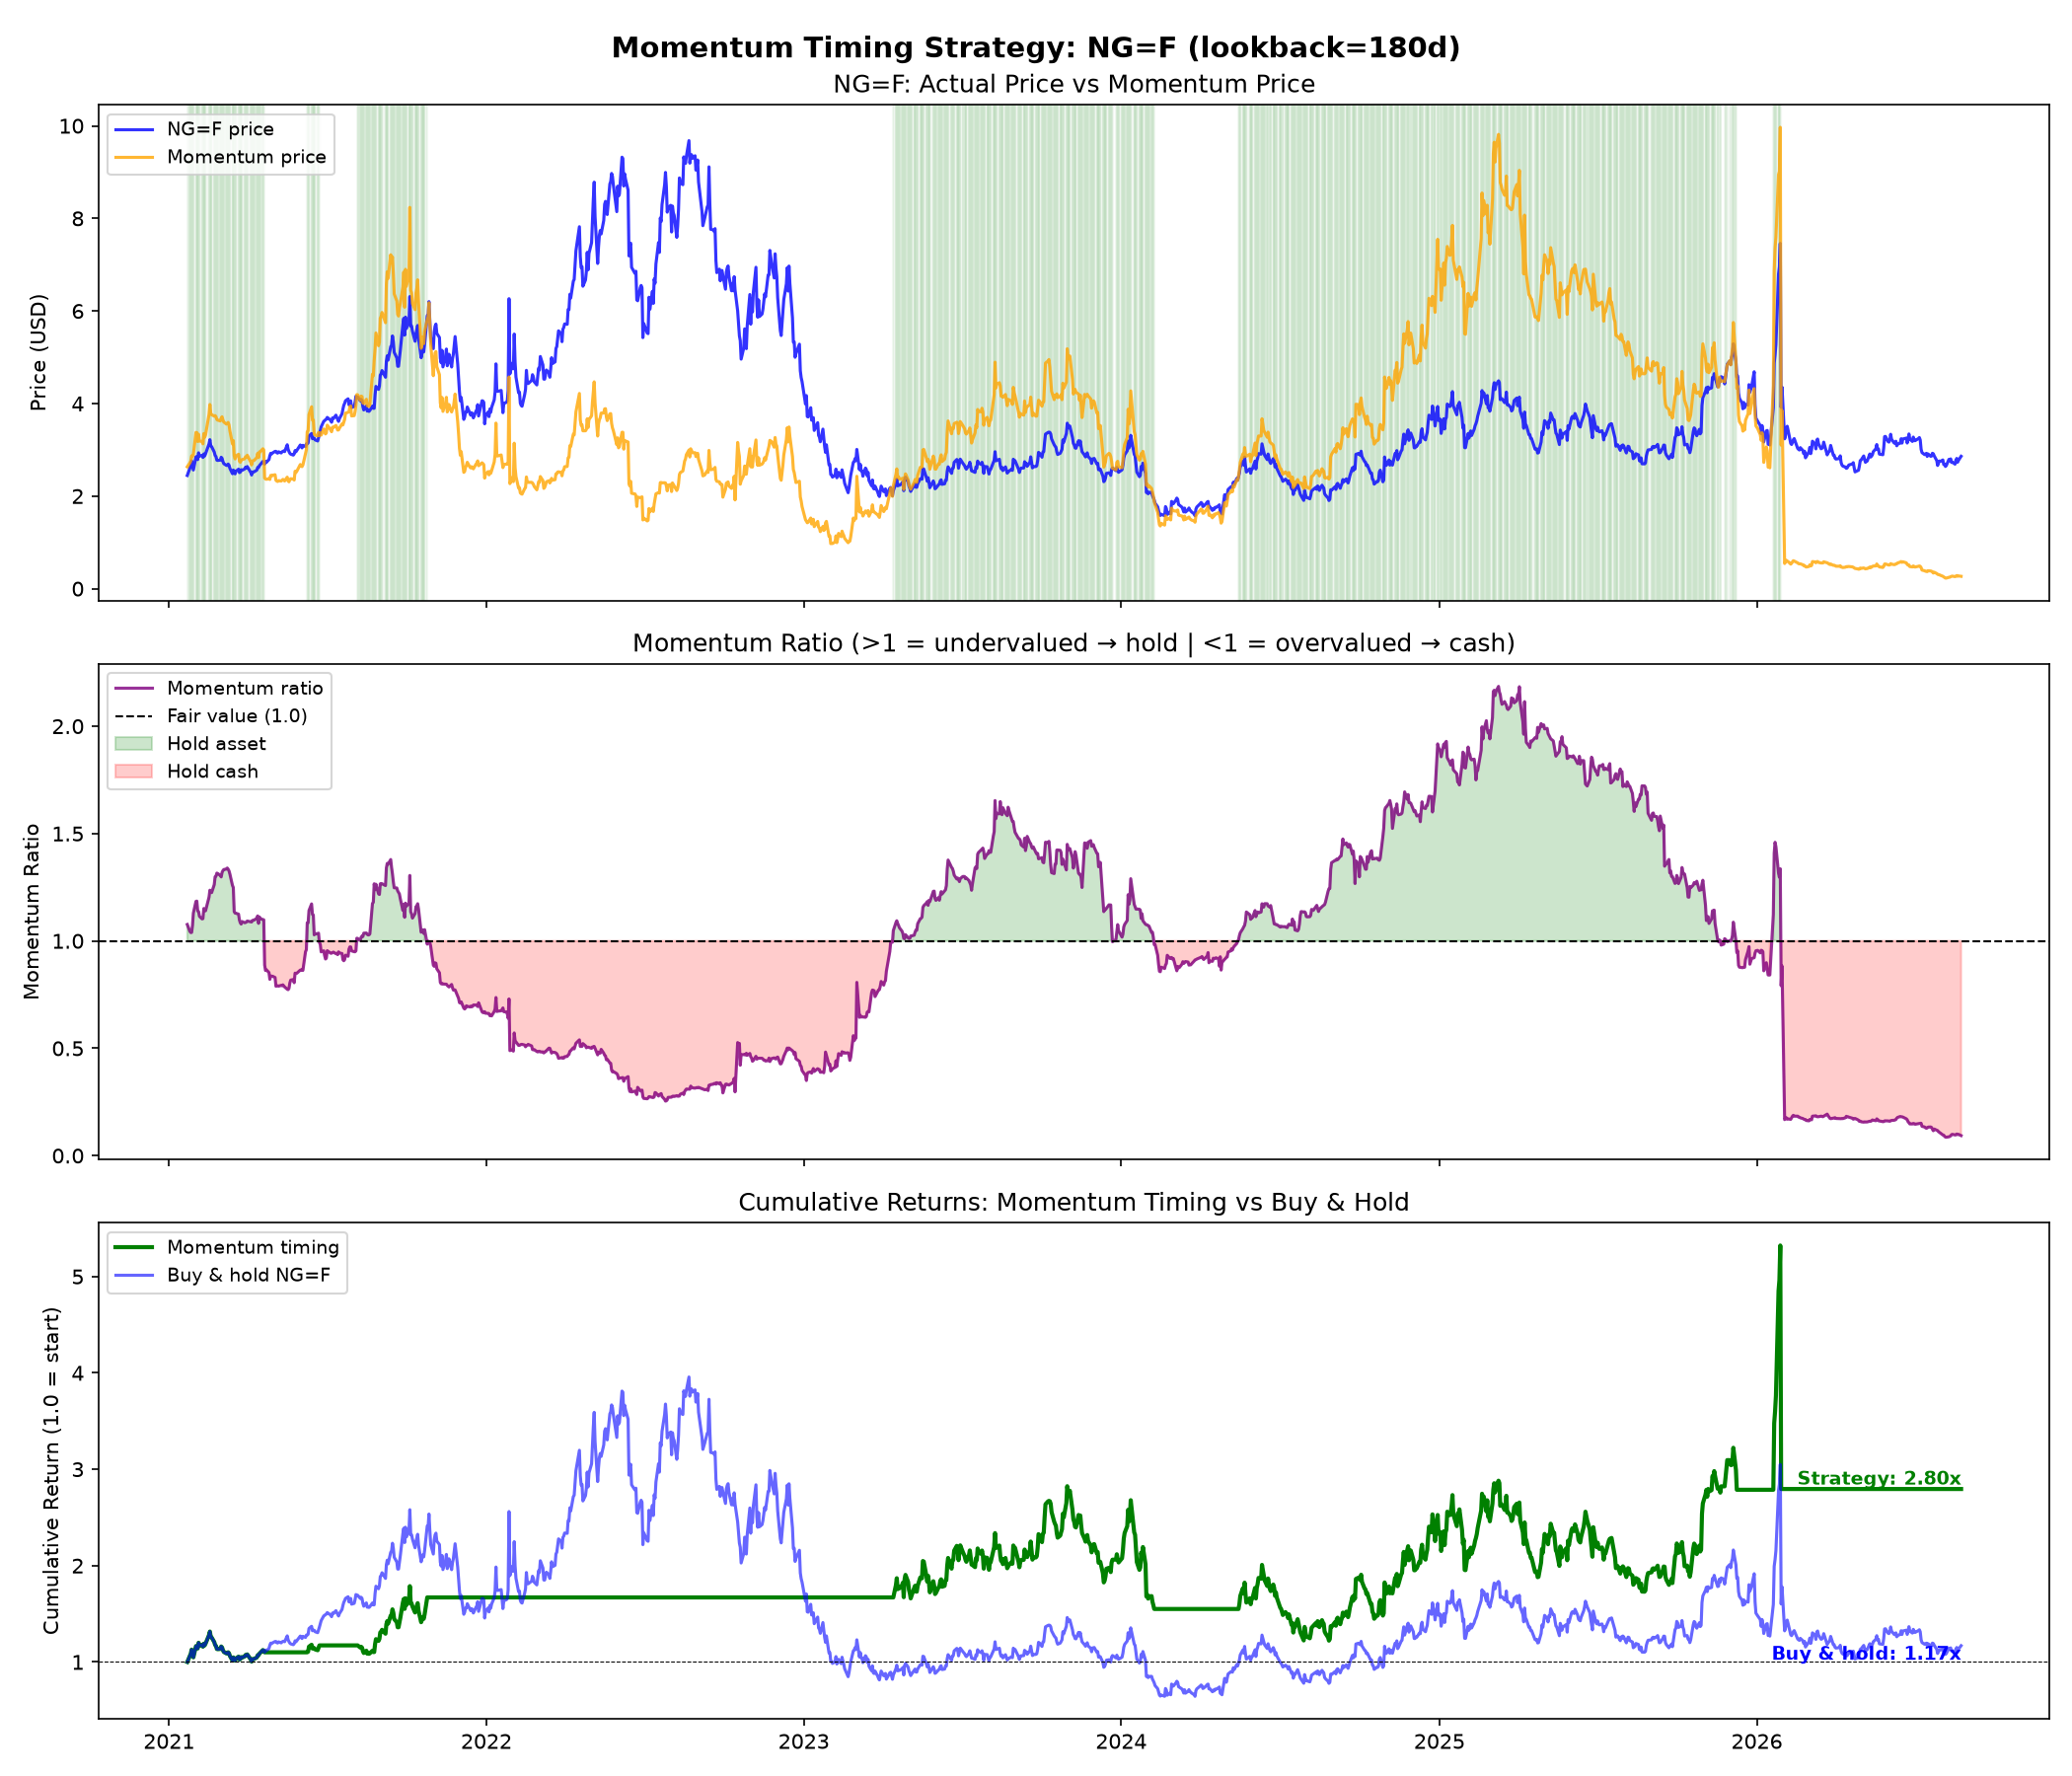
\includegraphics[width=\textwidth]{timing_NG=F.png}
    \caption{Natural gas: the most volatile commodity tested. The
    model captures the 2021--2022 spike and exits before the 83\%
    crash.}
\end{figure}

\subsection{Results}

\vspace{0.5em}
\begin{tabular}{@{}lrrr@{}}
    \toprule
    \textbf{Metric} & \textbf{90-day} & \textbf{180-day} & \textbf{365-day} \\
    \midrule
    Strategy return    & \textcolor{green}{\textbf{+309.9\%}} & $+179.5\%$ & $+88.4\%$  \\
    Buy \& hold return & $+10.7\%$  & $+16.9\%$  & $+3.9\%$   \\
    Alpha              & \textcolor{green}{\textbf{+299.2\%}} & $+162.6\%$ & $+84.4\%$ \\
    Sharpe ratio       & $0.90$     & $0.75$     & $0.61$     \\
    Max drawdown       & $-53.0\%$  & $-56.7\%$  & $-60.1\%$  \\
    Buy \& hold DD     & $-83.7\%$  & $-83.7\%$  & $-83.7\%$  \\
    Trades             & 17         & 11         & 2          \\
    Win rate           & 53\%       & 73\%       & 100\%      \\
    Avg win            & $+25.6\%$  & $+20.4\%$  & $+37.3\%$  \\
    Avg loss           & $-5.7\%$   & $-16.5\%$  & ---        \\
    \bottomrule
\end{tabular}

\begin{resultbox}[Verdict: Natural Gas --- Strong]{strong}
Natural gas is \textbf{the only asset where all three lookbacks
produce positive alpha}: 90-day +299\%, 180-day +163\%, 365-day +84\%.
Max drawdown cut from \textbf{$-83.7\%$ to $-53$--$60\%$}.

Natural gas is \emph{violently} volatile but structurally trendless
(buy \& hold returned only +17\% over 5 years). The momentum model
turns a flat, terrifying asset into a +180--310\% return by catching
spikes and avoiding collapses. This is the model's ideal environment:
\textbf{high volatility with no secular trend to fight}.
\end{resultbox}

\newpage

% ══════════════════════════════════════════════════════════════════
% PART VI: INDUSTRIAL METALS
% ══════════════════════════════════════════════════════════════════

\part{Industrial Metals}

\section{Copper (HG=F): 2021--2026}

\begin{figure}[H]
    \centering
    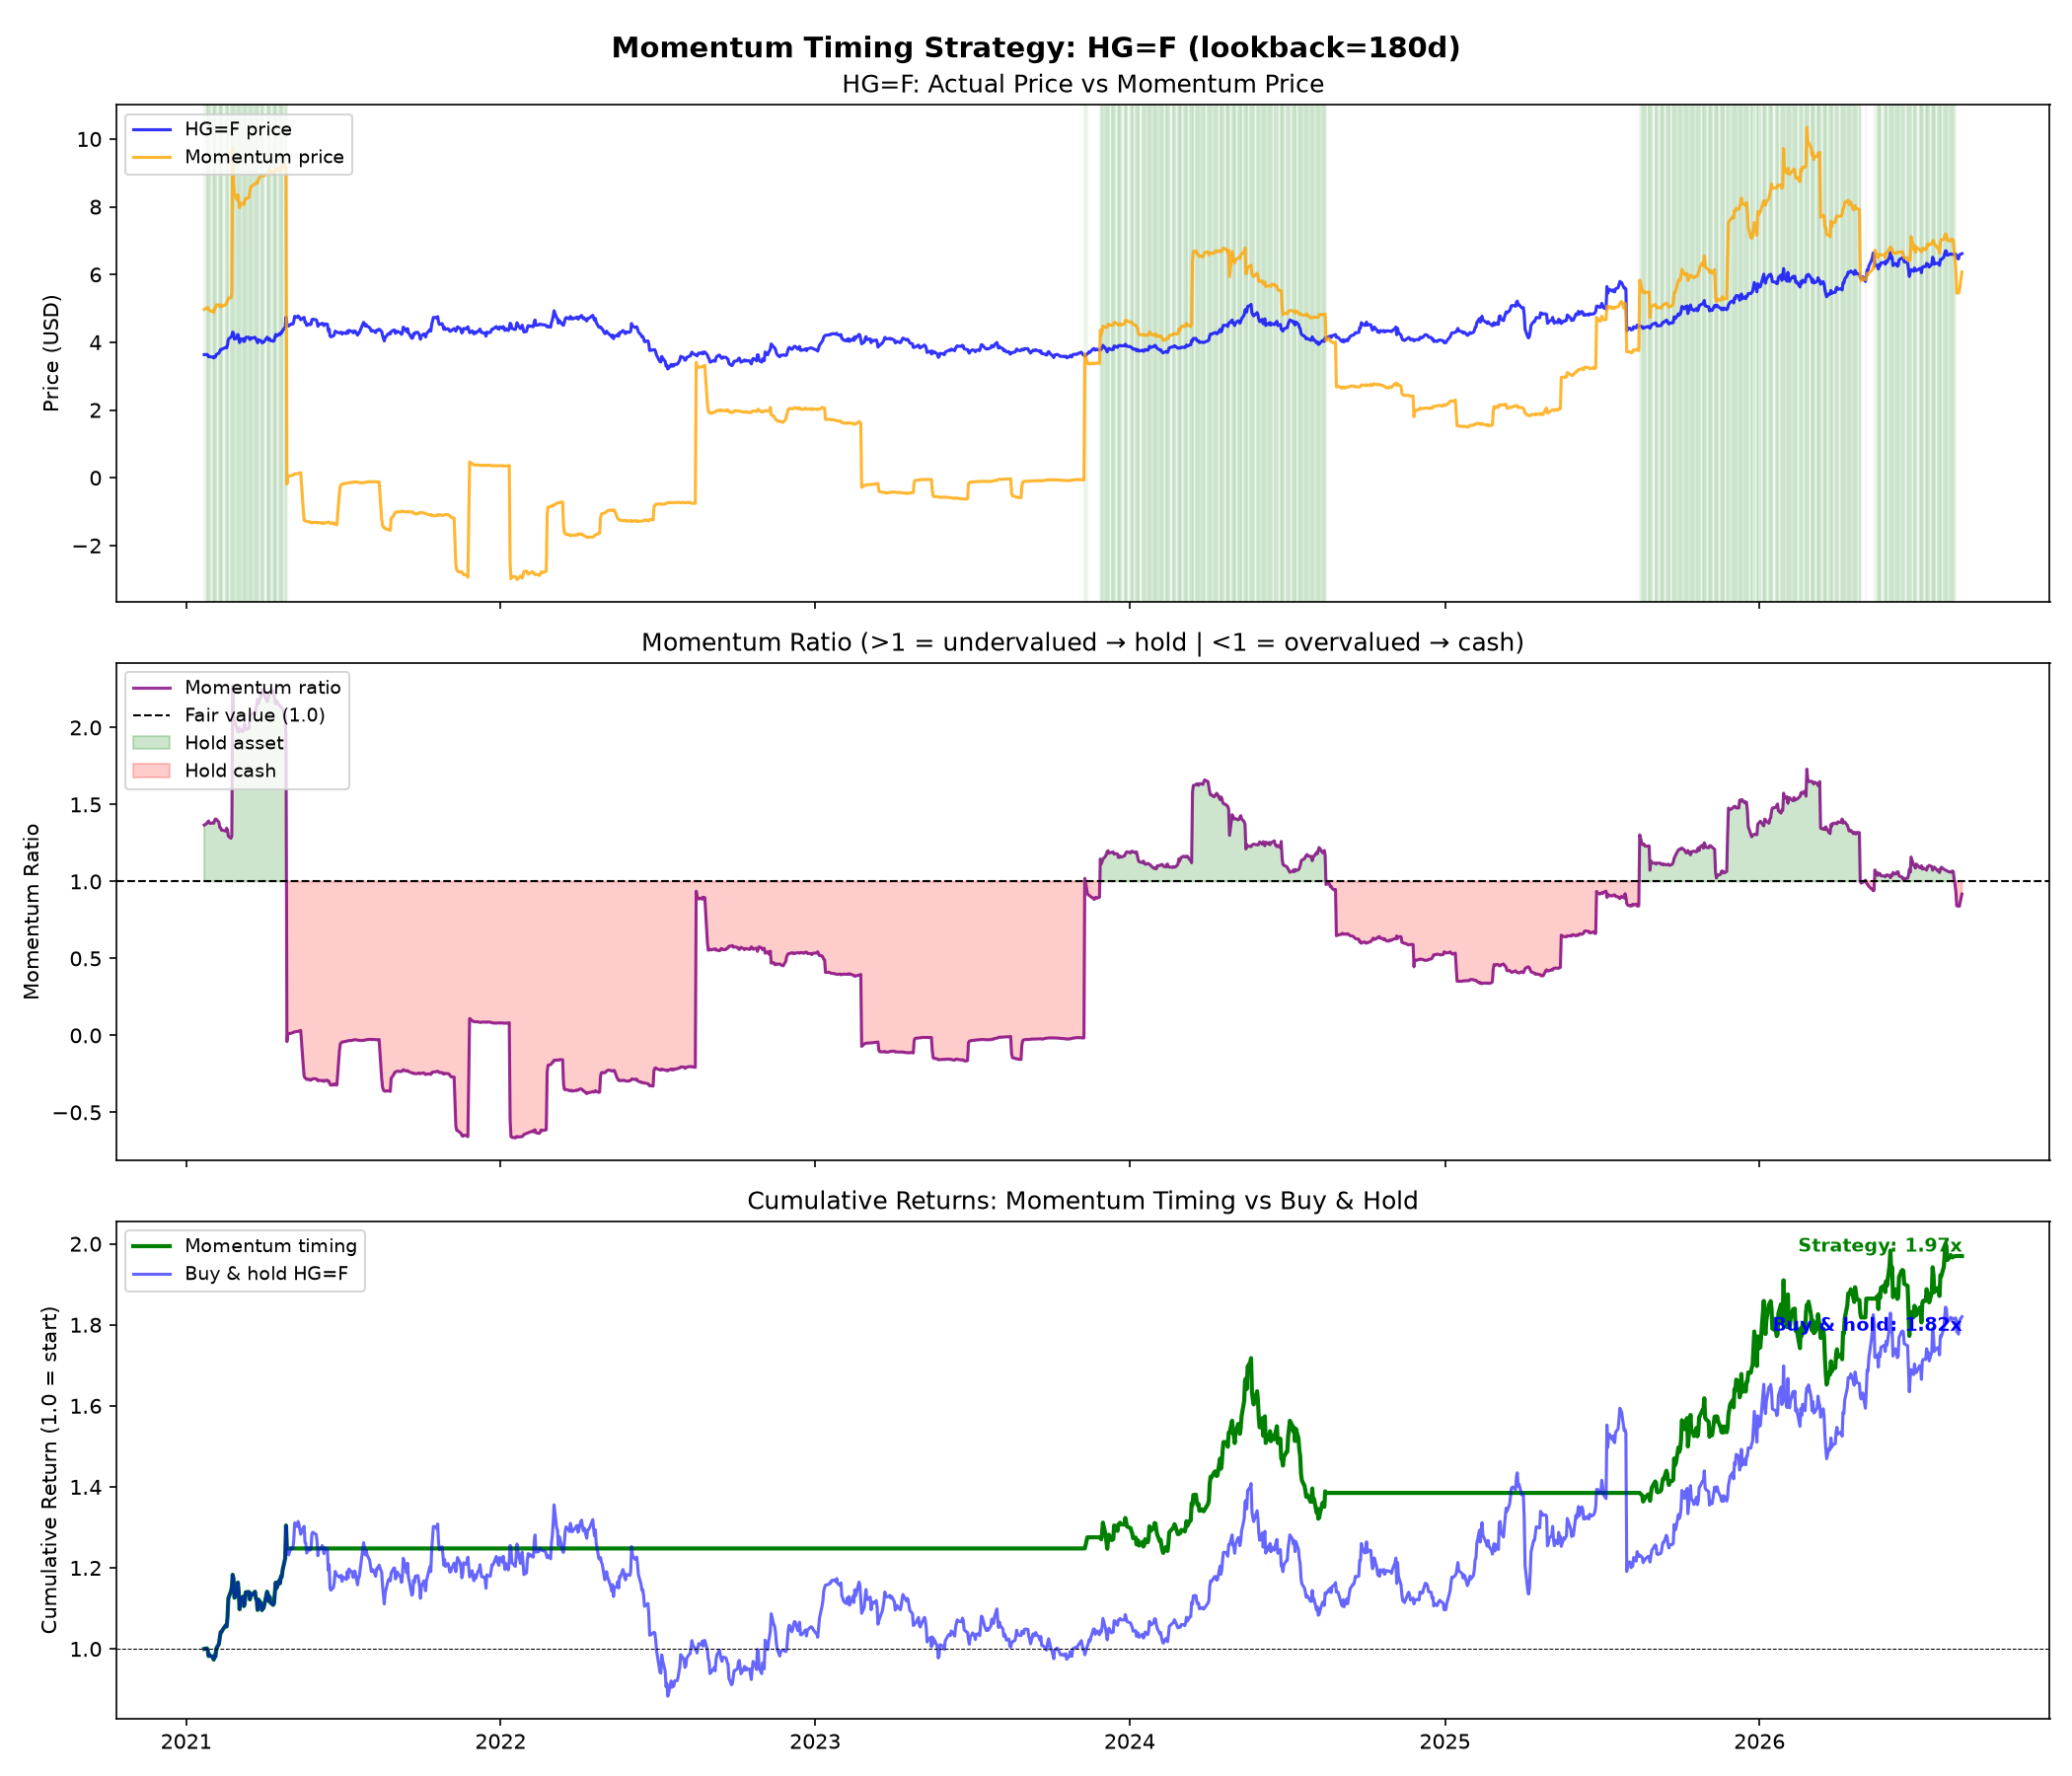
\includegraphics[width=\textwidth]{timing_HG=F.png}
    \caption{Copper: steady outperformance with minimal drawdown.
    The model catches the 2024--2025 commodity rally while avoiding
    the 2022 tightening-driven decline.}
\end{figure}

\subsection{Results}

\vspace{0.5em}
\begin{tabular}{@{}lrrr@{}}
    \toprule
    \textbf{Metric} & \textbf{90-day} & \textbf{180-day} & \textbf{365-day} \\
    \midrule
    Strategy return    & $+116.9\%$ & $+97.0\%$  & $+15.0\%$  \\
    Buy \& hold return & $+86.2\%$  & $+82.0\%$  & $+55.7\%$  \\
    Alpha              & \textcolor{green}{\textbf{+30.6\%}} & $+15.0\%$ & $-40.7\%$ \\
    Sharpe ratio       & $0.96$     & \textcolor{green}{\textbf{1.05}} & $0.41$ \\
    Max drawdown       & $-25.3\%$  & $-23.1\%$  & $-11.4\%$  \\
    Buy \& hold DD     & $-34.9\%$  & $-34.9\%$  & $-34.9\%$  \\
    Trades             & 10         & 6          & 4          \\
    Win rate           & 80\%       & 100\%      & 50\%       \\
    Avg win            & $+10.5\%$  & $+12.3\%$  & $+5.8\%$   \\
    Avg loss           & $-3.4\%$   & ---        & $-0.7\%$   \\
    \bottomrule
\end{tabular}

\begin{resultbox}[Verdict: Copper --- Quiet Achiever]{strong}
Copper is the \textbf{quiet achiever}: Sharpe 1.05 (third-highest
after SOL and BTC), \textbf{100\% win rate} (6/6 trades at 180d),
max drawdown consistently cut from $-35\%$ to $-11$--$25\%$.

Copper occupies a middle ground: more volatile than forex, less
volatile than crypto. The model extracts steady, reliable alpha
without the stomach-churning drawdowns of SOL or natgas.
\textbf{If you want momentum timing with the least stress, copper
is the answer.}
\end{resultbox}

\newpage

% ══════════════════════════════════════════════════════════════════
% PART VII: EQUITY INDEX
% ══════════════════════════════════════════════════════════════════

\part{Equity Index}

\section{S\&P 500 Futures (ES=F): 2021--2026}

\begin{figure}[H]
    \centering
    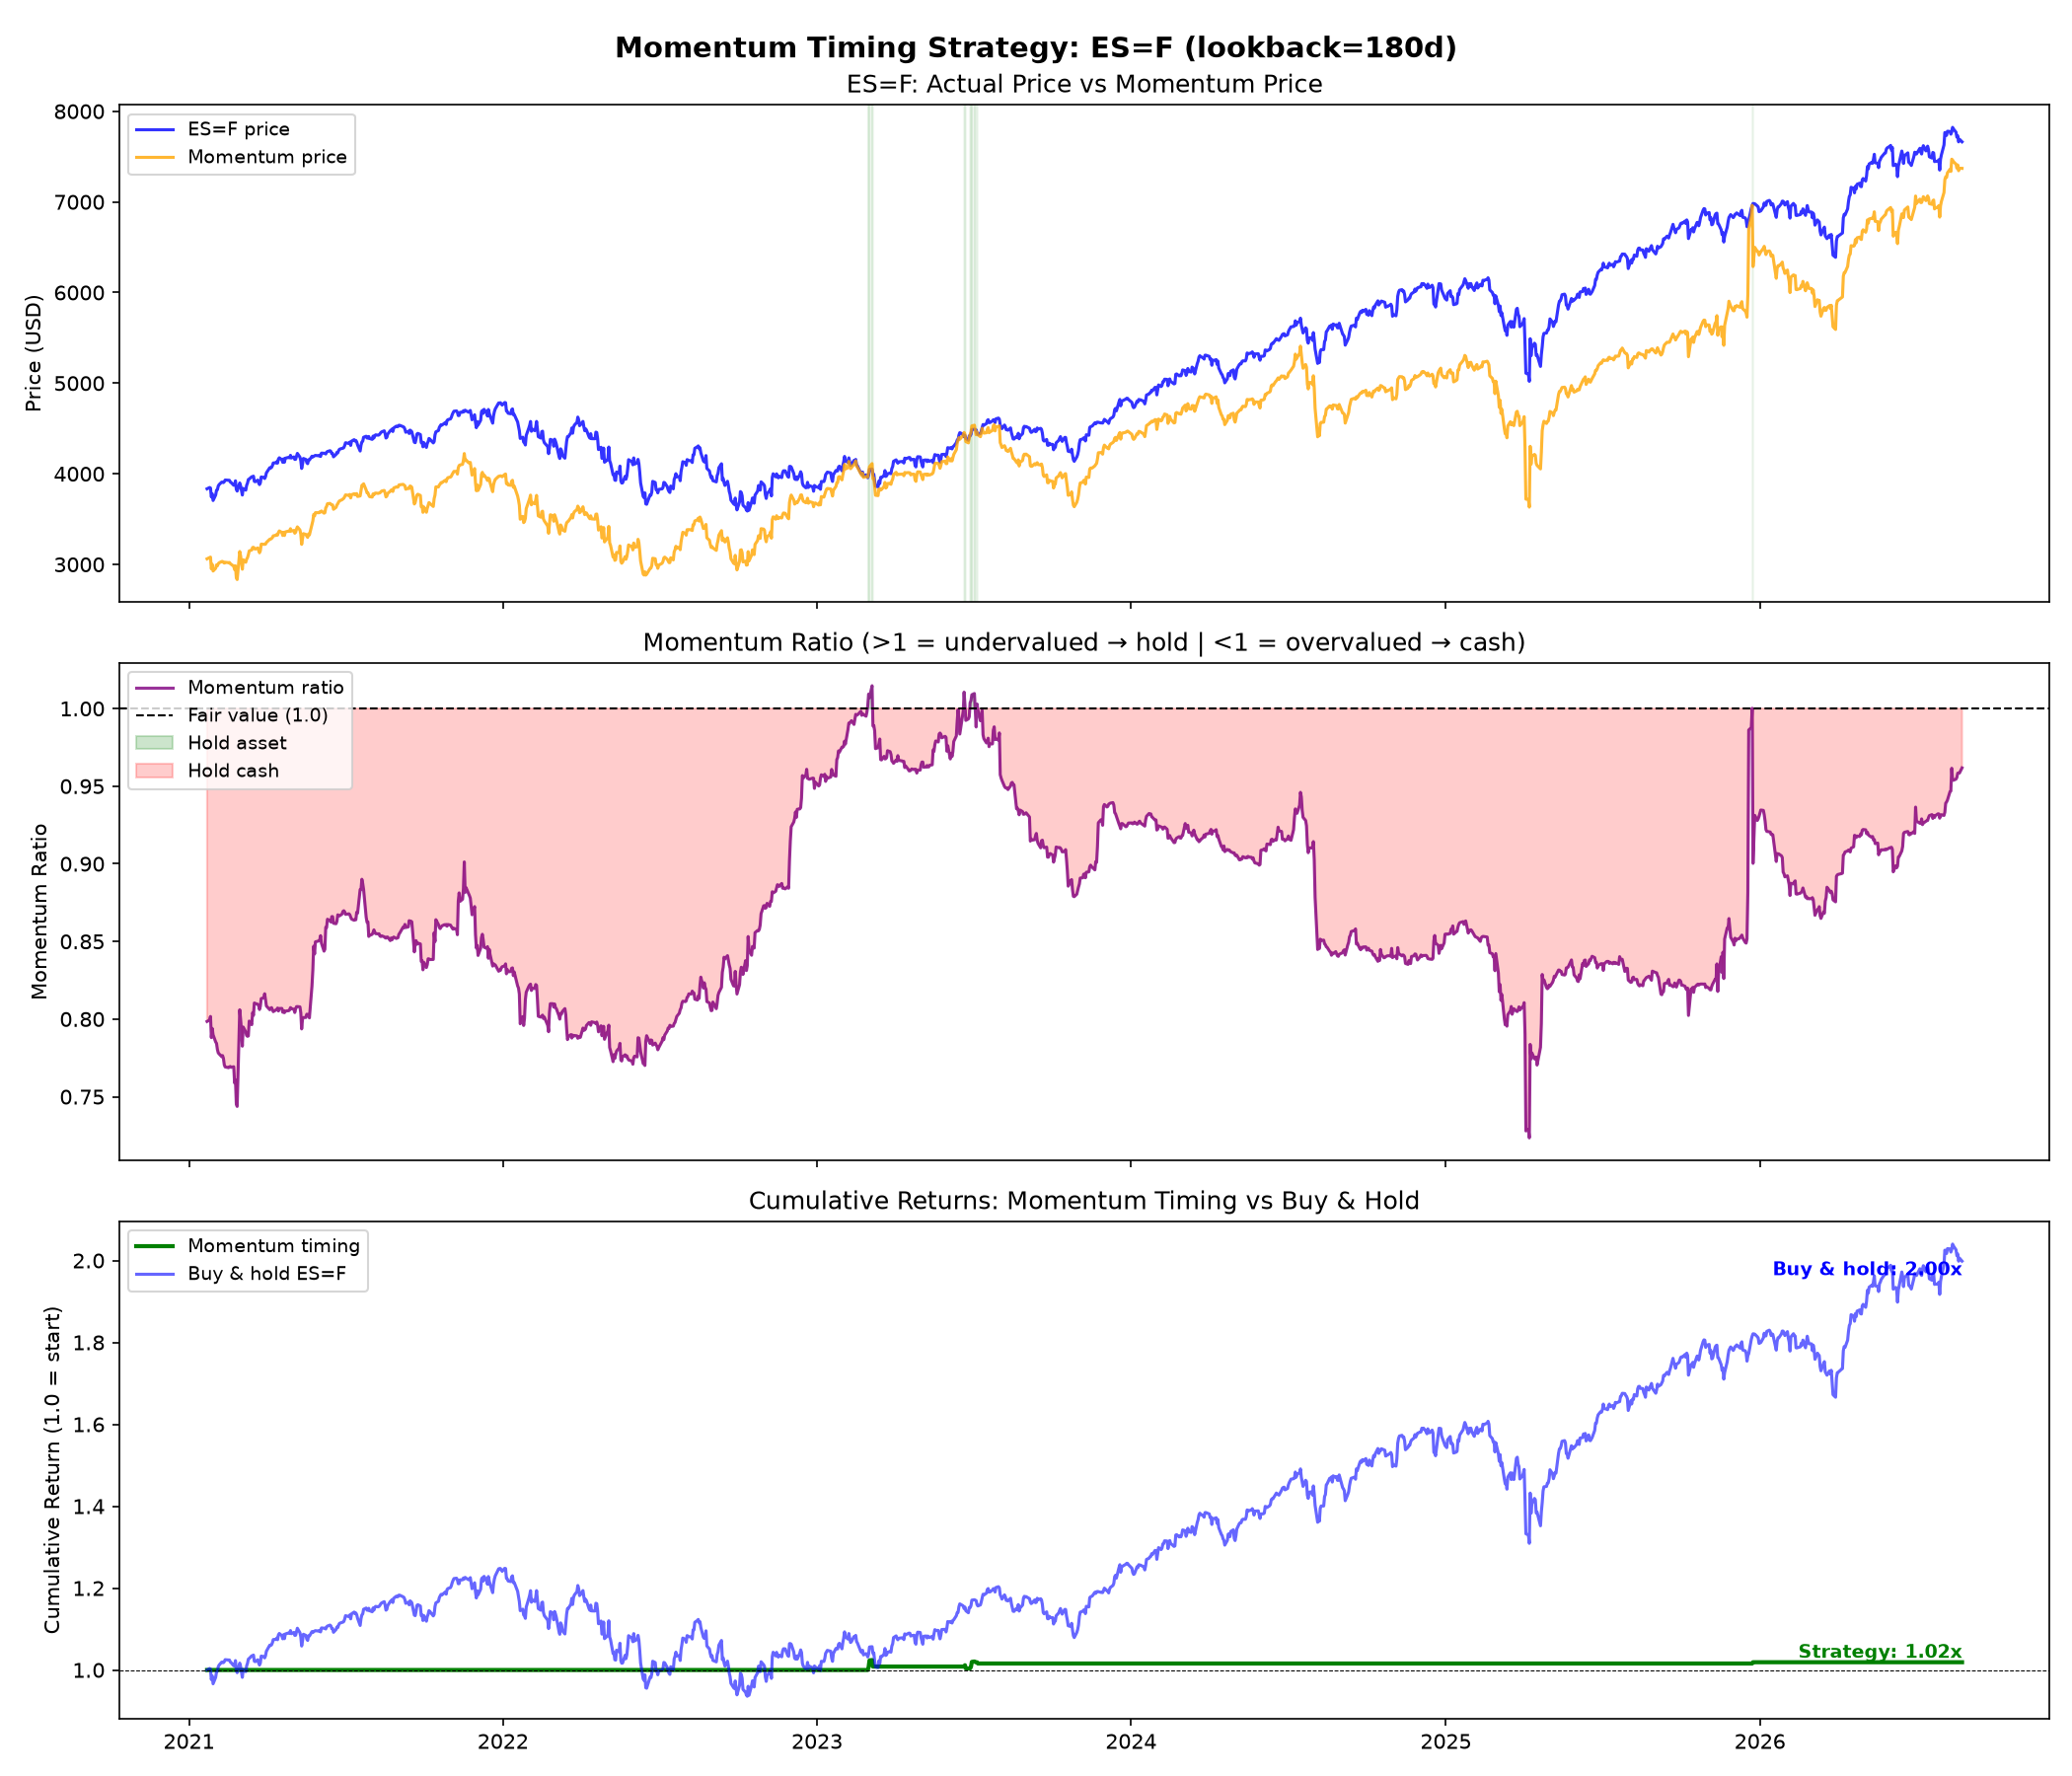
\includegraphics[width=\textwidth]{timing_ES=F.png}
    \caption{S\&P 500 futures: the model almost never enters the
    market. The momentum ratio stays below 1.0 for 99\% of the
    period, producing a flat green line while the index doubles.}
\end{figure}

\subsection{Results}

\vspace{0.5em}
\begin{tabular}{@{}lr@{}}
    \toprule
    \textbf{Metric} & \textbf{180-day} \\
    \midrule
    Strategy return    & $+1.9\%$   \\
    Buy \& hold return & $+99.9\%$  \\
    Alpha              & \textcolor{red}{\textbf{$-98.0\%$}} \\
    Sharpe ratio       & $0.34$     \\
    Max drawdown       & $-2.0\%$   \\
    Buy \& hold DD     & $-25.0\%$  \\
    Days in asset      & 0.9\%      \\
    Trades             & 5          \\
    Win rate           & 60\%       \\
    \bottomrule
\end{tabular}

\begin{resultbox}[Verdict: S\&P 500 --- Broken]{fail}
The S\&P 500 fails for a structural reason: \textbf{equity indices
have a permanent upward drift} driven by earnings growth, buybacks,
and index rebalancing. Volume is highest on \emph{down} days (panic
selling, margin calls), while up days have moderate volume (steady
accumulation). The pool model reads this as ``the big money is
bearish'' and keeps the momentum ratio below 1.0.

\textbf{Do not use this model on equity indices.}
\end{resultbox}

\newpage

% ══════════════════════════════════════════════════════════════════
% PART VIII: CROSS-ASSET COMPARISON & CONCLUSIONS
% ══════════════════════════════════════════════════════════════════

\part{Conclusions}

\section{Cross-Asset Comparison}

All results using best lookback (180d unless noted). All periods 5 years
(2021--2026) except gold and silver (16 years from 2010).

\vspace{0.5em}
{\small
\begin{tabular}{@{}lrrrrrrrrr@{}}
    \toprule
    & \textbf{SOL} & \textbf{BTC} & \textbf{NatGas} & \textbf{Copper} & \textbf{Oil} & \textbf{Silver} & \textbf{Gold} & \textbf{EUR} & \textbf{ES} \\
    & \textbf{(180d)} & \textbf{(180d)} & \textbf{(90d)} & \textbf{(180d)} & \textbf{(90d)} & \textbf{(16yr)} & \textbf{(16yr)} & \textbf{(180d)} & \textbf{(180d)} \\
    \midrule
    Strategy    & \textcolor{green}{\textbf{+7691}} & \textcolor{green}{\textbf{+463}} & \textcolor{green}{\textbf{+310}} & $+97$  & $+111$ & $+259$ & $+152$ & $+7$  & $+2$  \\
    Buy\&hold   & $+5094$ & $+168$ & $+11$  & $+82$  & $+79$  & $+310$ & $+334$ & $-4$  & $+100$ \\
    Alpha       & \textcolor{green}{\textbf{+2597}} & \textcolor{green}{\textbf{+295}} & \textcolor{green}{\textbf{+299}} & $+15$  & $+32$  & $-51$  & $-182$ & $+11$ & $-98$ \\
    \midrule
    Sharpe      & \textcolor{green}{\textbf{1.34}} & \textcolor{green}{\textbf{1.16}} & $0.90$ & \textcolor{green}{\textbf{1.05}} & $0.81$ & $0.54$ & $0.66$ & $0.30$ & $0.34$ \\
    Max DD      & $-79\%$ & $-28\%$ & $-53\%$ & $-23\%$ & $-34\%$ & $-47\%$ & $-25\%$ & $-8\%$ & $-2\%$ \\
    B\&H DD     & $-96\%$ & $-77\%$ & $-84\%$ & $-35\%$ & $-55\%$ & $-76\%$ & $-44\%$ & $-22\%$ & $-25\%$ \\
    \midrule
    Days in     & 55\%   & 34\%   & 50\%   & 35\%   & 29\%   & 40\%   & 36\%   & 53\%  & 1\%   \\
    Win rate    & 50\%   & 62\%   & 53\%   & 100\%  & 62\%   & 67\%   & 60\%   & 55\%  & 60\%  \\
    \bottomrule
\end{tabular}
}

\vspace{0.5em}
{\small All returns in \%. Best lookback chosen per asset.}

\vspace{1em}

\subsection{What Works}

\begin{enumerate}[leftmargin=2em]
    \item \textbf{SOL is the strongest result in the entire study.}
          +2597\% alpha, Sharpe 1.34, 18:1 win/loss asymmetry. Extreme
          volatility is the model's fuel.

    \item \textbf{Natural gas has positive alpha on all lookbacks.}
          The only asset to achieve this. A structurally trendless,
          violently volatile asset is the model's ideal environment.

    \item \textbf{BTC remains the flagship.} +295\% alpha, Sharpe
          1.16, 14:1 win/loss ratio. The most tradeable result because
          crypto markets are 24/7 with deep liquidity.

    \item \textbf{Copper is the best risk-adjusted commodity.} Sharpe
          1.05, 100\% win rate (6/6 trades). Lower alpha but much
          lower stress.

    \item \textbf{180 days is optimal for most assets.} Exception:
          energy commodities (oil, natgas), where 90 days captures
          faster-moving geopolitical and seasonal regimes.

    \item \textbf{Drawdown reduction is universal.} Every single asset
          tested --- even the failures --- shows reduced max drawdown
          vs buy \& hold. The model is better at telling you
          \emph{when to get out} than when to get in.

    \item \textbf{Win/loss asymmetry is universal.} Average wins are
          always much larger than average losses. The model cuts losers
          fast and lets winners run.

    \item \textbf{Forex: positive alpha on all six pairs.} Best used
          as a risk overlay, not a return strategy.
\end{enumerate}

\subsection{What Doesn't Work}

\begin{enumerate}[leftmargin=2em]
    \item \textbf{Equity indices (S\&P 500).} The structural upward
          drift keeps the momentum ratio permanently below 1.0. The
          model sits in cash 99\% of the time.
    \item \textbf{Pairs trading} between correlated assets (BTC/ETH).
          The model needs independent fundamentals.
    \item \textbf{ETH timing.} Volume data is too noisy.
    \item \textbf{Gold over long periods.} Extended sideways markets
          generate whipsaw losses.
    \item \textbf{365-day lookback on most assets.} Too slow to
          capture regime shifts. Exception: natural gas, where it
          still produces +84\% alpha.
    \item \textbf{Forex as a return strategy.} Returns are too small
          to justify trading costs.
\end{enumerate}

\section{Caveats}

\begin{enumerate}[leftmargin=2em]
    \item \textbf{Backtest $\neq$ live trading.} These results assume
          execution at the daily close with no slippage or fees.

    \item \textbf{Small samples.} 10--30 trades is not statistically
          robust. Strong alpha may be driven by a few large wins.

    \item \textbf{Volume data quality.} Crypto exchanges inflate
          volume through wash trading. The signal may be noisier than
          it appears.

    \item \textbf{No transaction costs.} Exchange fees (0.1--0.5\%
          per trade) and bid-ask spreads will reduce returns.

    \item \textbf{Tax implications.} Each trade is a taxable event.
          Frequent trading creates short-term capital gains at your
          marginal rate.

    \item \textbf{Survivor bias.} We tested BTC and gold because they
          went up. We would not have tested assets that went to zero.

    \item \textbf{Regime change.} Market structures evolve. The
          volume dynamics that produced these signals may not persist.
\end{enumerate}

\section{Recommendations}

If you had to pick trades from all the results:

\begin{enumerate}[leftmargin=2em]
    \item \textbf{Primary: SOL with 180-day momentum timing.}
          Highest alpha (+2597\%), best Sharpe (1.34). Extreme
          volatility makes it high-risk but the model tames it.
    \item \textbf{Core: BTC with 180-day momentum timing.}
          Most tradeable: deep liquidity, 24/7 markets, Sharpe 1.16.
    \item \textbf{Commodity: Natural gas with 90-day timing.}
          +299\% alpha on a structurally flat asset. Positive alpha
          on all lookbacks --- the model's ideal environment.
    \item \textbf{Conservative: Copper with 180-day timing.}
          Sharpe 1.05, 100\% win rate, lowest stress. The grown-up
          trade.
    \item \textbf{Risk overlay: Gold/Silver with 180-day timing.}
          Won't beat buy \& hold, but halves your drawdown.
\end{enumerate}

\subsection{Next Steps}

\begin{enumerate}[leftmargin=2em]
    \item \textbf{Paper trade.} Run the 180-day signal in real-time
          for 3--6 months on BTC, SOL, copper, and natgas. No real
          money.
    \item \textbf{Fine-tune lookback.} Test 120, 150, 200 days on
          BTC/SOL; test 60, 90, 120 days on energy commodities.
    \item \textbf{Add transaction costs} to the simulation.
    \item \textbf{Multi-asset portfolio.} Run BTC + copper + natgas
          simultaneously with capital allocation rules.
    \item \textbf{If confirmed:} Kraken/Coinbase for crypto (CCXT
          library). Interactive Brokers for commodity futures (CL, NG,
          HG). Gold and silver via ETFs (GLD, SLV).
\end{enumerate}

\vspace{2em}
\begin{center}
\textit{--- Robin}
\end{center}

\newpage

% ══════════════════════════════════════════════════════════════════
% APPENDIX: SOURCE CODE
% ══════════════════════════════════════════════════════════════════

\appendix
\part*{Appendix: Source Code}
\addcontentsline{toc}{part}{Appendix: Source Code}

All code lives in \texttt{$\sim$/git/andy/crypto/}. Python 3.8+,
no exchange account needed for backtesting.

\section{Setup}

\begin{codebox}[Shell]
\begin{lstlisting}[style=shell]
cd ~/git/andy/crypto
python3 -m venv venv
source venv/bin/activate
pip install yfinance pandas numpy matplotlib
\end{lstlisting}
\end{codebox}

\section{momentum\_single.py --- Complete File}

This is the main script. It handles everything: data fetching,
momentum calculation, simulation, reporting, and charting.

\begin{codebox}[momentum\_single.py]
\begin{lstlisting}[style=python]
"""
Momentum timing: single-asset directional strategy.

Uses the bookmaker-pool momentum model to time entries and exits.
Hold the asset when momentum price > actual price. Go to cash
when momentum price < actual price.

All data from yfinance (free, no auth).

Usage:
  python momentum_single.py                         # BTC, defaults
  python momentum_single.py --asset ETH-USD         # ETH
  python momentum_single.py --asset GC=F            # Gold futures
  python momentum_single.py --asset SI=F            # Silver futures
  python momentum_single.py --lookback 90 --plot    # 90-day + charts
  python momentum_single.py --start 2010-01-01      # custom period
"""

import argparse
import os
import numpy as np
import pandas as pd
import yfinance as yf
from datetime import datetime, timedelta
import matplotlib
matplotlib.use("Agg")
import matplotlib.pyplot as plt

SCRIPT_DIR = os.path.dirname(os.path.abspath(__file__))


# -- Core algorithm: Bookmaker Pool --------------------------------

def compute_rolling_momentum(history, lookback_days):
    """
    Compute rolling momentum price using the bookmaker pool model.

    For each day, takes a window of `lookback_days` history, runs
    the pool model, and records the resulting momentum price and
    ratio (momentum_price / actual_price).

    Volume is normalised (divided by window mean) to prevent
    overflow on crypto and commodity volumes.
    """
    closes = history["Close"].values
    volumes = history["Volume"].values
    dates = history.index

    momentum_prices = [np.nan] * len(history)
    momentum_ratios = [np.nan] * len(history)

    for i in range(lookback_days, len(history)):
        window_close = closes[i - lookback_days:i + 1]
        window_vol = volumes[i - lookback_days:i + 1]

        if len(window_close) < 10:
            continue

        # Daily returns within the window
        returns = np.diff(window_close) / window_close[:-1]
        vols = window_vol[1:]

        # Normalise volume to prevent overflow
        mean_vol = vols.mean()
        if mean_vol == 0:
            continue
        norm_vols = vols / mean_vol

        # Net flow = normalised_volume * return
        net_flows = norm_vols * returns

        # Run the bookmaker pool
        pool = float(window_close[0])
        mp = pool

        for j in range(len(net_flows)):
            pool += net_flows[j] * mp
            mp = pool

        momentum_prices[i] = mp
        momentum_ratios[i] = mp / closes[i]

    result = pd.DataFrame({
        "Close": closes,
        "MomentumPrice": momentum_prices,
        "MomentumRatio": momentum_ratios,
    }, index=dates)

    return result.dropna()


# -- Simulation ----------------------------------------------------

def simulate_timing(asset_symbol, lookback_days,
                    start_date, end_date):
    """
    Simulate the timing strategy.

    Rule:
      - If MomentumRatio > 1.0: hold the asset
      - If MomentumRatio <= 1.0: hold cash

    Uses previous day's signal (no lookahead bias).
    """
    fetch_start = start_date - timedelta(
        days=lookback_days + 60)

    print(f"Fetching {asset_symbol}...")
    ticker = yf.Ticker(asset_symbol)
    hist = ticker.history(
        start=fetch_start, end=end_date, interval="1d")
    print(f"  Got {len(hist)} days")

    if hist.empty:
        raise ValueError(f"No data for {asset_symbol}")

    print(f"Computing rolling momentum "
          f"(lookback={lookback_days} days)...")
    df = compute_rolling_momentum(hist, lookback_days)

    # Trim to simulation period
    start_ts = pd.Timestamp(start_date)
    if df.index.tz is not None:
        start_ts = start_ts.tz_localize(df.index.tz)
    df = df[df.index >= start_ts]

    if df.empty:
        raise ValueError("No data in simulation period")

    # Signal: 1 = hold asset, 0 = hold cash
    df["signal"] = (
        df["MomentumRatio"] > 1.0).astype(int)

    # Position: use previous day's signal
    df["position"] = (
        df["signal"].shift(1).fillna(0).astype(int))

    # Returns
    df["asset_return"] = (
        df["Close"].pct_change().fillna(0))
    df["strategy_return"] = (
        df["position"] * df["asset_return"])

    # Cumulative
    df["cumulative_asset"] = (
        (1 + df["asset_return"]).cumprod())
    df["cumulative_strategy"] = (
        (1 + df["strategy_return"]).cumprod())

    return df


# -- Reporting -----------------------------------------------------

def print_report(df, asset_symbol, lookback_days):
    """Print backtest summary with trade analysis."""
    total_days = len(df)
    days_in = (df["position"] == 1).sum()
    days_out = (df["position"] == 0).sum()

    total_return = (
        df["cumulative_strategy"].iloc[-1] - 1) * 100
    asset_return = (
        df["cumulative_asset"].iloc[-1] - 1) * 100

    transitions = (
        df["position"].diff().abs() > 0).sum()

    # Sharpe (annualised, 365 days)
    sr = df["strategy_return"]
    sharpe = (sr.mean() / sr.std() * np.sqrt(365)
              if sr.std() > 0 else 0)

    # Max drawdown
    cummax = df["cumulative_strategy"].cummax()
    drawdown = (
        df["cumulative_strategy"] - cummax) / cummax
    max_dd = drawdown.min() * 100

    bh_cummax = df["cumulative_asset"].cummax()
    bh_drawdown = (
        df["cumulative_asset"] - bh_cummax) / bh_cummax
    bh_max_dd = bh_drawdown.min() * 100

    # Trade-level analysis
    in_blocks = []
    block_start = None
    for i in range(len(df)):
        if (df["position"].iloc[i] == 1
                and block_start is None):
            block_start = i
        elif (df["position"].iloc[i] == 0
                and block_start is not None):
            ret = (df["Close"].iloc[i]
                   / df["Close"].iloc[block_start]
                   - 1) * 100
            in_blocks.append(ret)
            block_start = None
    if block_start is not None:
        ret = (df["Close"].iloc[-1]
               / df["Close"].iloc[block_start]
               - 1) * 100
        in_blocks.append(ret)

    wins = sum(1 for r in in_blocks if r > 0)
    losses = sum(1 for r in in_blocks if r <= 0)
    avg_win = (np.mean([r for r in in_blocks if r > 0])
               if wins > 0 else 0)
    avg_loss = (np.mean([r for r in in_blocks if r <= 0])
                if losses > 0 else 0)

    # Crashes avoided
    out_blocks = []
    block_start = None
    for i in range(len(df)):
        if (df["position"].iloc[i] == 0
                and block_start is None):
            block_start = i
        elif (df["position"].iloc[i] == 1
                and block_start is not None):
            avoided = (df["Close"].iloc[i]
                       / df["Close"].iloc[block_start]
                       - 1) * 100
            out_blocks.append(avoided)
            block_start = None
    if block_start is not None:
        avoided = (df["Close"].iloc[-1]
                   / df["Close"].iloc[block_start]
                   - 1) * 100
        out_blocks.append(avoided)

    crashes_avoided = sum(
        1 for r in out_blocks if r < -10)

    sym = asset_symbol[:3]
    print()
    print("=" * 60)
    print(f"MOMENTUM TIMING: {asset_symbol}")
    print("=" * 60)
    print(f"  Period:  "
          f"{df.index[0].strftime('%Y-%m-%d')} -> "
          f"{df.index[-1].strftime('%Y-%m-%d')}")
    print(f"  Lookback: {lookback_days} days")
    print(f"  Days in {sym}: {days_in} "
          f"({days_in/total_days*100:.1f}%)")
    print(f"  Days cash:  {days_out} "
          f"({days_out/total_days*100:.1f}%)")
    print(f"  Trades: {len(in_blocks)}")
    print()
    print(f"  Strategy:  {total_return:+.1f}%")
    print(f"  Buy&Hold:  {asset_return:+.1f}%")
    print(f"  Alpha:     "
          f"{total_return - asset_return:+.1f}%")
    print(f"  Sharpe:    {sharpe:.2f}")
    print(f"  Max DD:    {max_dd:.1f}% "
          f"(hold: {bh_max_dd:.1f}%)")
    if in_blocks:
        print(f"  Win rate:  "
              f"{wins}/{len(in_blocks)} "
              f"({wins/len(in_blocks)*100:.0f}%)")
        print(f"  Avg win:   {avg_win:+.1f}%  "
              f"Avg loss: {avg_loss:+.1f}%")
    print(f"  Crashes avoided: {crashes_avoided}")
    print()

    return {
        "total_return": total_return,
        "asset_return": asset_return,
        "sharpe": sharpe,
        "max_dd": max_dd,
        "bh_max_dd": bh_max_dd,
        "trades": len(in_blocks),
        "wins": wins, "losses": losses,
        "avg_win": avg_win, "avg_loss": avg_loss,
    }


# -- Charting ------------------------------------------------------

def plot_results(df, asset_symbol, lookback_days,
                 stats, tag=""):
    """Generate 3-panel chart."""
    fig, axes = plt.subplots(
        3, 1, figsize=(14, 12), sharex=True)

    # Panel 1: Price vs momentum price
    ax = axes[0]
    ax.plot(df.index, df["Close"],
            label=f"{asset_symbol} price",
            color="blue", alpha=0.8)
    ax.plot(df.index, df["MomentumPrice"],
            label="Momentum price",
            color="orange", alpha=0.8)
    for i in range(1, len(df)):
        if df["position"].iloc[i] == 1:
            ax.axvspan(df.index[i-1], df.index[i],
                       alpha=0.05, color="green")
    ax.set_ylabel("Price (USD)")
    ax.set_title(f"{asset_symbol}: "
                 f"Actual Price vs Momentum Price")
    ax.legend(loc="upper left", fontsize=9)

    # Panel 2: Momentum ratio
    ax = axes[1]
    ax.plot(df.index, df["MomentumRatio"],
            label="Momentum ratio",
            color="purple", alpha=0.8)
    ax.axhline(y=1.0, color="black", linewidth=1,
               linestyle="--", label="Fair value (1.0)")
    ax.fill_between(
        df.index, df["MomentumRatio"], 1.0,
        where=df["MomentumRatio"] > 1.0,
        alpha=0.2, color="green", label="Hold asset")
    ax.fill_between(
        df.index, df["MomentumRatio"], 1.0,
        where=df["MomentumRatio"] < 1.0,
        alpha=0.2, color="red", label="Hold cash")
    ax.set_ylabel("Momentum Ratio")
    ax.set_title("Momentum Ratio "
                 "(>1 = hold | <1 = cash)")
    ax.legend(loc="upper left", fontsize=9)

    # Panel 3: Cumulative returns
    ax = axes[2]
    ax.plot(df.index, df["cumulative_strategy"],
            label="Momentum timing",
            color="green", linewidth=2)
    ax.plot(df.index, df["cumulative_asset"],
            label=f"Buy & hold {asset_symbol}",
            color="blue", alpha=0.6)
    ax.axhline(y=1.0, color="black",
               linewidth=0.5, linestyle="--")

    sf = df["cumulative_strategy"].iloc[-1]
    hf = df["cumulative_asset"].iloc[-1]
    ax.annotate(f"Strategy: {sf:.2f}x",
                xy=(df.index[-1], sf),
                fontsize=9, fontweight="bold",
                color="green", ha="right", va="bottom")
    ax.annotate(f"Buy & hold: {hf:.2f}x",
                xy=(df.index[-1], hf),
                fontsize=9, fontweight="bold",
                color="blue", ha="right", va="top")

    ax.set_ylabel("Cumulative Return")
    ax.set_title("Cumulative Returns: "
                 "Timing vs Buy & Hold")
    ax.legend(loc="upper left", fontsize=9)

    fig.suptitle(
        f"Momentum Timing: {asset_symbol} "
        f"(lookback={lookback_days}d)",
        fontsize=14, fontweight="bold")
    fig.tight_layout()

    out = os.path.join(
        SCRIPT_DIR,
        f"timing_{asset_symbol.replace('-','')}"
        f"{tag}.png")
    fig.savefig(out, dpi=150)
    plt.close(fig)
    print(f"Saved: {out}")
    return out


# -- CLI -----------------------------------------------------------

def main():
    parser = argparse.ArgumentParser(
        description="Momentum timing backtest")
    parser.add_argument(
        "--asset", default="BTC-USD",
        help="Ticker symbol. Examples: BTC-USD, "
             "ETH-USD, GC=F (gold), SI=F (silver)")
    parser.add_argument(
        "--lookback", type=int, default=180,
        help="Lookback window in days (default: 180)")
    parser.add_argument(
        "--start", default=None,
        help="Start date YYYY-MM-DD (default: 5yr ago)")
    parser.add_argument(
        "--end", default=None,
        help="End date YYYY-MM-DD (default: today)")
    parser.add_argument(
        "--plot", action="store_true",
        help="Generate PNG charts")

    args = parser.parse_args()

    end_date = (
        datetime.strptime(args.end, "%Y-%m-%d")
        if args.end else datetime.now())
    start_date = (
        datetime.strptime(args.start, "%Y-%m-%d")
        if args.start else
        end_date - timedelta(days=5*365))

    print(f"\n  Asset:    {args.asset}")
    print(f"  Lookback: {args.lookback} days")
    print(f"  Period:   "
          f"{start_date.strftime('%Y-%m-%d')} -> "
          f"{end_date.strftime('%Y-%m-%d')}\n")

    df = simulate_timing(
        args.asset, args.lookback,
        start_date, end_date)

    stats = print_report(
        df, args.asset, args.lookback)

    if args.plot:
        plot_results(
            df, args.asset, args.lookback, stats)

    csv_out = os.path.join(
        SCRIPT_DIR,
        f"timing_{args.asset.replace('-','')}.csv")
    df.to_csv(csv_out)
    print(f"Saved: {csv_out}")


if __name__ == "__main__":
    main()
\end{lstlisting}
\end{codebox}

\section{Running the Experiments}

\begin{codebox}[Reproduce all results from this report]
\begin{lstlisting}[style=shell]
# Bitcoin (5 years, 3 lookback windows)
python momentum_single.py --asset BTC-USD --lookback 90 \
       --start 2021-01-01 --plot
python momentum_single.py --asset BTC-USD --lookback 180 \
       --start 2021-01-01 --plot
python momentum_single.py --asset BTC-USD --lookback 365 \
       --start 2021-01-01 --plot

# Ethereum
python momentum_single.py --asset ETH-USD --lookback 180 \
       --start 2021-01-01 --plot

# Solana (5 years, 3 lookback windows)
python momentum_single.py --asset SOL-USD --lookback 90 \
       --start 2021-01-01 --plot
python momentum_single.py --asset SOL-USD --lookback 180 \
       --start 2021-01-01 --plot
python momentum_single.py --asset SOL-USD --lookback 365 \
       --start 2021-01-01 --plot

# Gold (16 years)
python momentum_single.py --asset GC=F --lookback 90 \
       --start 2010-01-01 --plot
python momentum_single.py --asset GC=F --lookback 180 \
       --start 2010-01-01 --plot
python momentum_single.py --asset GC=F --lookback 365 \
       --start 2010-01-01 --plot

# Silver (16 years)
python momentum_single.py --asset SI=F --lookback 90 \
       --start 2010-01-01 --plot
python momentum_single.py --asset SI=F --lookback 180 \
       --start 2010-01-01 --plot
python momentum_single.py --asset SI=F --lookback 365 \
       --start 2010-01-01 --plot

# Recent period only (gold & silver)
python momentum_single.py --asset GC=F --lookback 180 \
       --start 2021-01-01 --plot
python momentum_single.py --asset SI=F --lookback 180 \
       --start 2021-01-01 --plot

# Crude Oil (5 years, 3 lookback windows)
python momentum_single.py --asset CL=F --lookback 90 \
       --start 2021-01-01 --plot
python momentum_single.py --asset CL=F --lookback 180 \
       --start 2021-01-01 --plot
python momentum_single.py --asset CL=F --lookback 365 \
       --start 2021-01-01 --plot

# Natural Gas (5 years, 3 lookback windows)
python momentum_single.py --asset NG=F --lookback 90 \
       --start 2021-01-01 --plot
python momentum_single.py --asset NG=F --lookback 180 \
       --start 2021-01-01 --plot
python momentum_single.py --asset NG=F --lookback 365 \
       --start 2021-01-01 --plot

# Copper (5 years, 3 lookback windows)
python momentum_single.py --asset HG=F --lookback 90 \
       --start 2021-01-01 --plot
python momentum_single.py --asset HG=F --lookback 180 \
       --start 2021-01-01 --plot
python momentum_single.py --asset HG=F --lookback 365 \
       --start 2021-01-01 --plot

# S&P 500 Futures (the failure case)
python momentum_single.py --asset ES=F --lookback 180 \
       --start 2021-01-01 --plot

# Forex futures (CME, 5 years)
python momentum_single.py --asset 6E=F --lookback 180 \
       --start 2021-01-01 --plot    # EUR
python momentum_single.py --asset 6A=F --lookback 180 \
       --start 2021-01-01 --plot    # AUD
python momentum_single.py --asset 6B=F --lookback 180 \
       --start 2021-01-01 --plot    # GBP
python momentum_single.py --asset 6J=F --lookback 180 \
       --start 2021-01-01 --plot    # JPY
python momentum_single.py --asset 6C=F --lookback 180 \
       --start 2021-01-01 --plot    # CAD
python momentum_single.py --asset 6S=F --lookback 180 \
       --start 2021-01-01 --plot    # CHF

# Try any yfinance ticker:
python momentum_single.py --asset AAPL --lookback 180 --plot
python momentum_single.py --asset BHP.AX --lookback 180 --plot
\end{lstlisting}
\end{codebox}

\end{document}
